\documentclass[12pt,a4paper]{article}
\usepackage[top=2.54cm,bottom=2.54cm,left=2.54cm,right=2.54cm]{geometry}
\usepackage{fontspec}
\usepackage{xeCJK}
\usepackage{array}
\usepackage{graphicx}
\usepackage{hyperref}
\usepackage{amsmath}
\usepackage{listings}
\usepackage{setspace}
\usepackage{indentfirst}

\setmainfont{Times New Roman}
\setsansfont{Arial}
\setmonofont{Menlo}
\setCJKmainfont[BoldFont=BiauKaiTC]{BiauKaiTC}
\setCJKsansfont{Heiti TC}
\setCJKmonofont{PingFang TC}
\XeTeXlinebreaklocale "zh"
\XeTeXlinebreakskip = 0pt plus 1pt
\hypersetup{hidelinks}
\sloppy
\setlength{\parindent}{2em}
\setlength{\parskip}{0pt}
\onehalfspacing
\renewcommand{\contentsname}{目錄}

\begin{document}
\pagenumbering{roman}
\begin{center}
{\LARGE\bfseries 國立彰化師範大學\\[0.6em]資訊工程學系碩士班\\[0.6em]碩士論文初稿}
\end{center}

\begin{center}
{\Large\bfseries 單房間非連網家電環境影響學習之稀疏感測空間數位孿生原型}
\end{center}

\begin{center}A Sparse-Sensing Spatial Digital Twin for Learning Environmental Impacts of Non-Networked Appliances in a Single Room\end{center}

\begin{center}研究生：林昀佑\end{center}

\begin{center}指導教授：易昶霈\end{center}

\begin{center}版本：論文初稿 v0.2\end{center}

\begin{center}日期：2026 年 4 月 15 日\end{center}

\clearpage

\section*{審定書}
\addcontentsline{toc}{section}{審定書}

國立彰化師範大學資訊工程學系碩士班


碩士論文審定書


單房間非連網家電環境影響學習之稀疏感測空間數位孿生原型


研究生：林昀佑


本論文業經審查及口試合格，特此證明。


論文考試委員會召集人：


委員：


委員：


指導教授：易昶霈 博士


所長：


中華民國 115 年 月


\clearpage

\section*{誌謝}
\addcontentsline{toc}{section}{誌謝}

本研究能夠完成，首先感謝指導教授易昶霈博士在研究方向、方法與寫作上的指導與支持，以及各位口試委員的指正與建議。感謝求學過程中幫助我的各位師長所提供的學習環境，也感謝家人的支持與包容。


林昀佑 謹誌於


國立彰化師範大學資訊工程學系（所）


中華民國 115 年 4 月


\clearpage

\section*{摘要}
\addcontentsline{toc}{section}{摘要}

智慧建築與智慧居家系統需要掌握室內環境狀態，才能支援舒適度評估、能源管理與設備控制。然而，實際房間中常見的冷氣、窗戶與照明往往沒有連網能力，也無法直接回報狀態；同時，房間內通常只能布建少量感測器，難以直接量測完整空間分布。這使得一般數位孿生若同時缺乏設備遙測與高密度量測，便難以對真實房間提供可用的環境估計與控制建議。


本研究以單一矩形房間為研究場域，提出一個基於有限角落感測器與連續影響場估計之三因子空間數位孿生原型。研究過程中，本研究先後比較純插值、僅局部影響場與資料驅動修正等作法，最終採用 bulk + local field 作為主模型，並以冷氣、窗戶與照明之參數化影響函數描述非連網裝置對不同區域的作用。系統固定使用 8 顆角落感測器，即天花板四角與地面四角，每個節點量測溫度、濕度與照度，並以感測器殘差進行主動設備 power scale 校準與 trilinear residual correction，以修正背景場與設備影響函數之偏差。在此基礎上，本研究再加入 hybrid residual neural network 延伸模組，以小型多層感知器學習主模型的剩餘誤差，而不直接取代原本的可解釋結構。


除空間場估計外，本研究亦建立裝置啟用前後感測資料之影響學習流程，透過最小平方法估計非連網裝置的環境影響係數，並根據目標區域的舒適度偏差輸出候選控制動作排序。為補足 direct source + obstruction 對照度間接回填亮度的低估，本研究另在 illuminance 路徑加入 lightweight single-bounce diffuse reflection 近似，以地板、天花板、牆面與啟用中的家具表面作為次級反射面。為提升系統可存取性，本研究另提供本地服務介面，其中包含 MCP server 與 web demo，作為同一套模型能力的工具化存取層。評估方面，本研究以 8 組標準情境、48 組窗戶矩陣、IDW baseline 比較與 hybrid residual held-out 測試驗證方法可行性；其中 base model 在標準情境下之平均 MAE 分別為溫度 0.0474、濕度 0.1764 與照度 2.1288，而加入 Fourier low-pass denoising 的 hybrid residual correction 在 held-out 情境下可進一步將 field MAE 降至溫度 0.0026、濕度 0.0040 與照度 0.1752。


關鍵字：空間數位孿生、稀疏感測、非連網家電、室內環境建模、溫度、濕度、照度、角落感測器。


\clearpage

\section*{Abstract}
\addcontentsline{toc}{section}{Abstract}

Smart building and smart home systems require indoor environmental awareness to support comfort assessment, energy management, and device control. In ordinary rooms, however, influential appliances such as conventional air conditioners, manual windows, and ordinary lights often expose no telemetry, while only a small number of sensors can be installed. As a result, practical room-scale digital twins must work with both sparse observations and incomplete device-state information.


This thesis proposes a sparse-sensing spatial digital twin for a single room. The final design is a reduced-order bulk-plus-local field model with parameterized appliance influence functions, active-device power calibration, and trilinear residual correction from eight corner sensors. The system further learns environmental impact coefficients of non-networked appliances from before-and-after sensor observations, ranks candidate control actions according to target-zone comfort improvement, and extends the base estimator with an optional hybrid residual neural correction layer instead of replacing the base model with an end-to-end black-box predictor.


The prototype is implemented in Python and exposed through a local service layer, including an MCP interface and a rotatable web demo, enabling interactive scenario queries, point-level estimation, baseline comparison, appliance-impact learning, and a 48-case window simulation matrix across time of day, weather, and season. A lightweight one-bounce diffuse reflection approximation is further added to the illuminance path so that floors, walls, ceilings, and active furniture surfaces can contribute indirect fill light without requiring full optical rendering. Across the canonical scenarios, the base model achieves average MAE of 0.0474 for temperature, 0.1764 for humidity, and 2.1288 for illuminance, while the hybrid residual layer with Fourier low-pass denoising on temperature and humidity residual traces further reduces held-out field MAE to 0.0026, 0.0040, and 0.1752, respectively. These results indicate that sparse corner sensing can still support an interpretable and trainable indoor twin when model structure, calibration, and learning are assigned to different layers.


Keywords: spatial digital twin, sparse sensing, non-networked appliances, indoor environment modeling, temperature, humidity, illuminance, corner sensors.


\clearpage

\section*{目錄}
\addcontentsline{toc}{section}{目錄}

摘要……I


Abstract……II


誌謝……III


目錄……IV


表目錄……V


圖目錄……VI


第一章 緒論…… 1


  1.1 研究背景…… 1


  1.2 研究動機…… 1


  1.3 研究問題…… 2


  1.4 研究範圍與限制…… 2


  1.5 預期貢獻…… 2


第二章 文獻探討…… 3


  2.1 室內環境建模…… 3


  2.2 空間插值與場估計…… 3


  2.3 數位孿生與智慧建築…… 3


  2.4 房間尺度室內因子實驗研究…… 4


  2.5 非連網裝置影響學習…… 4


  2.6 MCP 與 AI Agent Tool Interface…… 5


  2.7 與相似研究之差異定位…… 5


  2.8 公開資料與訓練資料適用性…… 6


第三章 系統架構與數學模型…… 7


  3.1 系統架構…… 7


  3.2 房間、區域與感測器設定…… 7


  3.3 三因子場模型…… 8


  3.4 設備影響函數…… 8


  3.5 感測器校正模型…… 9


  3.6 非連網裝置影響學習…… 9


  3.7 訓練資料組裝流程…… 9


  3.8 Hybrid Residual Neural Network 延伸…… 10


  3.9 控制動作排序…… 10


第四章 系統實作與服務介面…… 11


  4.1 Python 原型…… 11


  4.2 MCP Tools…… 11


  4.3 Gemma/Ollama Bridge…… 12


  4.4 Web Demo…… 12


第五章 模擬案例與結果分析…… 13


  5.1 標準情境設定…… 13


  5.2 場重建誤差…… 13


  5.3 IDW Baseline 比較…… 14


  5.4 非連網裝置影響學習…… 14


  5.5 窗戶時段、天氣、季節矩陣與直接輸入…… 14


  5.6 Hybrid Residual Neural Network 結果…… 14


  5.7 公開資料集 Task-Aligned Benchmark 結果…… 15


  5.8 研究過程與實作挑戰…… 18


  5.9 可旋轉 3D 展示…… 18


第六章 結論與未來工作…… 19


  6.1 結論…… 19


  6.2 研究限制…… 19


  6.3 未來工作…… 19


參考文獻…… 20


附錄…… 22


\clearpage

\section*{表目錄}
\addcontentsline{toc}{section}{表目錄}

表 2-1 相似研究差異比較…… 5


表 2-2 公開資料集概覽與適用性…… 6


表 2-3 Task-aligned benchmark 設計…… 6


表 3-1 房間與感測器設定…… 7


表 3-2 訓練資料表格說明…… 9


表 4-1 核心模組一覽…… 11


表 5-1 標準情境結果摘要…… 13


表 5-2 IDW 與本研究 field MAE 比較…… 14


表 5-3 窗戶矩陣情境節選…… 15


表 5-4 SML2010 Benchmark 結果…… 16


表 5-5 CU-BEMS Benchmark 結果…… 17


\clearpage

\section*{圖目錄}
\addcontentsline{toc}{section}{圖目錄}

圖 3-1 系統整體分層架構…… 7


圖 3-2 主要執行資料流…… 7


圖 3-3 房間感測器與目標區域配置…… 8


圖 3-4 感測器校正與影響學習流程…… 9


圖 5-1 驗證與實驗流程…… 13


圖 5-2 三裝置同時作用溫度場 3D 點雲（all\_\allowbreak{}active）…… 13


圖 5-3 僅冷氣作用溫度場 3D 點雲（ac\_\allowbreak{}only）…… 14


圖 5-4 僅燈具作用照度場 3D 點雲（light\_\allowbreak{}only）…… 14


圖 5-5 三裝置全開溫度場 3D 點雲（5.9 節）…… 18


圖 5-6 僅開窗溫度場 3D 點雲（window\_\allowbreak{}only）…… 18


圖 5-7 僅燈具照度場 3D 點雲（light\_\allowbreak{}only，5.9 節）…… 18


\clearpage

\clearpage\pagenumbering{arabic}

\section*{第一章 緒論}
\addcontentsline{toc}{section}{第一章 緒論}

\subsection*{1.1 研究背景}

智慧家庭與智慧建築系統逐漸被用於室內環境監控、能源管理與舒適度控制。這類系統通常需要知道空間中溫度、濕度與照度的分布，才能判斷使用者所在區域是否過熱、過暗或過於潮濕。然而，實際房間內不可能在每一個位置都布建感測器，因此系統往往只能取得少量離散點位資料。若僅依賴單點或少數點位量測，容易忽略同一空間中不同區域的環境差異。


另一方面，許多既有家電並不是智慧裝置。傳統冷氣、一般開關照明或手動窗戶可能無法連網，也無法主動回報開關狀態、出力或作用範圍。這些裝置雖然無法被直接讀取，卻會持續改變室內環境。若數位孿生模型只依賴智慧裝置 API，將無法完整描述一般房間中的環境變化。因此，本研究關注的核心問題是：如何透過有限感測器觀測資料，學習非連網裝置對空間環境造成的影響，並將此學習結果用於更準確的三因子控制推薦。


\subsection*{1.2 研究動機}

在原型開發初期，本研究曾嘗試將問題簡化為角落感測器插值或純局部影響場疊加，但很快發現兩個問題。第一，若只靠插值，模型雖能平滑填補空間，卻無法表達冷氣出風方向、窗邊日照或燈具位置等設備語意；第二，若只做局部場疊加，則容易出現設備附近變化明顯、全室平均狀態卻不合理的結果。這些實作經驗直接促成後續的 bulk + local field 架構、感測器校正流程，以及只把神經網路放在 residual correction 層的設計。


\begin{itemize}
\item 只知道角落感測器數值時，仍需要估計房間中央、靠窗區與門側區的三因子狀態。
\item 裝置沒有連網時，仍希望從環境變化中推估它是否對空間造成影響。
\item 新增或啟用冷氣、窗戶、照明後，系統應能估計其對不同區域造成的變化。
\item 學習裝置影響後，模型應能支援開冷氣、開窗或開燈等候選控制動作排序。
\item 將模型封裝為標準化工具介面後，AI client 或 agent 可查詢與使用數位孿生能力。
\end{itemize}

\subsection*{1.3 研究問題}

\begin{itemize}
\item RQ1：在只有 8 顆角落感測器的條件下，是否能建立單房間溫度、濕度與照度的空間估計模型？
\item RQ2：在家電或環境裝置沒有連網狀態回報的情況下，是否能從環境感測資料學習其對空間不同區域的影響？
\item RQ3：學習後的裝置影響模型，是否能依三因子偏差輸出候選控制動作排序，例如選擇開冷氣、開窗或開燈？
\item RQ4：將數位孿生模型封裝為標準化工具介面後，是否能讓 AI client 查詢、模擬與使用控制推薦能力？
\end{itemize}

\subsection*{1.4 研究範圍與限制}

\begin{itemize}
\item 研究場域固定為單一矩形房間，不處理多房間或跨空間空氣交換。
\item 感測器配置固定為天花板四角與地面四角，共 8 顆角落節點。
\item 設備類型聚焦於冷氣、窗戶與照明。
\item 模型為簡化動態模型，不追求 CFD 等級高精度流場。
\item 濕度保留於模型中，但作為次核心變數處理。
\item 控制功能只做候選動作排序，不做自動閉環控制。
\item MCP 部分定位為本地 stdio server 與 AI-agent-accessible interface，不宣稱提出新的 MCP protocol。
\end{itemize}

\subsection*{1.5 預期貢獻}

\begin{itemize}
\item 提出一個以單房間、8 顆角落感測器為前提的三因子空間數位孿生原型，明確描述 temperature、humidity 與 illuminance 場。
\item 建立包含 bulk + local field、active device power calibration、trilinear correction 與裝置影響學習的可解釋估測流程。
\item 建立訓練資料組裝與 hybrid residual correction 路線，使真實感測資料可用於參數校正、影響學習與殘差修正，而非直接取代主模型。
\item 提出可對接 MCP、Web demo 與公開資料集 task-aligned benchmark 的研究原型與評估框架。
\end{itemize}

\clearpage

\section*{第二章 文獻探討}
\addcontentsline{toc}{section}{第二章 文獻探討}

\subsection*{2.1 室內環境建模}

室內環境建模的主要目的，在於描述空間中熱舒適、能源使用與設備控制之間的關係。高精度方法如 computational fluid dynamics（CFD）雖可細緻描述空氣流動、傳熱與邊界交換，但通常需要大量幾何細節、材料參數與邊界條件，計算成本亦相對較高。相較之下，reduced-order model、grey-box thermal model 與控制導向動態模型著重於以較少參數捕捉主要動態，並保留參數辨識與即時推估能力，因此更適合用於建築控制、預測與數位孿生原型 [1][2][3]。基於此，本研究不追求 CFD 等級的高解析流場，而採用偏向控制導向與可解釋性的簡化空間模型。


\subsection*{2.2 空間插值與場估計}

在感測器數量有限的情況下，最直接的方法是使用空間插值估計未量測位置。本研究採用 inverse distance weighting（IDW）作為 baseline。IDW 的優點是實作簡單且不依賴設備先驗，但其估計完全由量測點距離決定，無法反映冷氣出風方向、窗戶位置、照明熱源或設備作用範圍等結構資訊。相較之下，zonal model 與 hybrid spatial model 提供了介於 well-mixed room model 與 CFD 之間的折衷途徑，可在維持較低計算成本的同時保留主要空間差異 [4][5][6]。因此，本研究將場模型設計為 bulk + local field：以 bulk state 描述房間整體平均狀態的時間收斂，以 local field 表示設備附近與特定區域的空間差異，藉此兼顧可解釋性與可計算性。


\subsection*{2.3 數位孿生與智慧建築}

數位孿生通常被視為實體系統在數位空間中的動態對應模型，其核心價值在於將感測資料、系統狀態與分析模型整合為可更新、可查詢且可推估的數位映射。在智慧建築領域中，數位孿生常與 BIM、IoT 感測、設備監控與能源管理系統結合，用於營運最佳化與狀態預測。近年的建築數位孿生回顧指出，多數研究著重於平台架構、資料整合與建築尺度的決策支援，但對於少量感測器條件下之單房間空間場重建與設備影響推估，討論仍相對有限 [7]。因此，本研究的定位並非建構完整 BIM/BMS 平台，而是針對單房間、低成本感測器與非連網裝置場景提出一個可運作的簡化數位孿生原型。


\subsection*{2.4 房間尺度室內因子實驗研究}

若將文獻範圍收斂到房間尺度的實驗研究，可以發現溫度、濕度與照度並不是彼此孤立的環境因子。Chinazzo 等人以 office-like test room 為實驗場域，控制不同室溫與日光照度條件，研究 visual perception 與 thermal perception 之間的交互作用，指出日照與室溫會共同影響受試者的感知結果 [18][19]。Lan 等人則在教室條件下同時調整熱環境與照明參數，分析其對學習表現與主觀感受的影響，顯示 thermal and visual environments 可在同一受控場域中被聯合操控與評估 [20]。這類研究雖不以數位孿生為主，但提供了重要前提：房間內三因子至少在實驗設計層級上具備共同量測與共同分析的必要性。


另一類與本研究更接近的工作，是冷氣、開窗或通風策略對房間環境的實驗或現地量測。Kuwahara 等人在大學實驗室中比較空調運轉與自然通風策略，量測溫度、相對濕度與 CO2 變化，用於評估室內環境與舒適 [21]。Zhou 等人則對綠建築辦公室進行長期 field study，追蹤 thermal environment、relative humidity、CO2 與 visual environment，並結合使用者滿意度調查 [22]。Wang 等人針對寒冷地區住宅建築的冬季室內環境品質進行實測，指出低能耗住宅中的室溫與相對濕度仍可能出現不理想分布 [23]。這些研究共同說明，房間尺度的 IEQ 實驗並不罕見，而且冷氣、通風與外氣條件確實會使房間內部環境產生可量測差異。


然而，現有房間尺度實驗研究多半聚焦於舒適評估、單一場域量測，或多因子對認知與滿意度的影響，較少進一步處理有限感測器下的空間場重建、非連網裝置影響學習，以及可被外部 AI 系統查詢的工具化服務。Geng 等人對綠建築辦公室進行大規模與長期 IEQ 比較，Lee 等人則分析研究機構中不同工作型態與 IEQ 的關係 [24][25]；這些研究證明房間內溫度、濕度、照度與舒適度之間具有實際研究基礎，但尚未形成單房間、三因子、8 顆角落感測器、設備影響學習與控制推薦整合於同一原型的做法。基於此，本研究並非宣稱房間室內因子實驗是全新問題，而是主張：本研究將既有 IEQ 實驗研究常見的環境因子量測，進一步推展為可估場、可校正、可學習與可服務化的單房間數位孿生方法。


\subsection*{2.5 非連網裝置影響學習}

既有智慧家庭與智慧建築研究，常預設設備可由網路介面直接讀取或控制。然而在一般居住空間中，傳統冷氣、手動窗戶與一般照明往往不具備可直接讀取的連網能力。此時，若系統仍希望掌握設備對環境的作用，就必須從感測到的環境變化反推設備影響。近期研究顯示，有限感測器搭配 data assimilation、hybrid model 或感測配置分析，確實能對室內溫濕度場進行重建，並評估量測點配置對重建品質的影響 [5][8][9]。本研究延續此方向，將裝置啟用前後的感測器差異視為學習訊號，並利用裝置空間影響基底與最小平方法估計其對溫度、濕度與照度的影響係數，以支援後續的場估計與控制推薦。


\subsection*{2.6 MCP 與 AI Agent Tool Interface}

Model Context Protocol（MCP）提供一種標準化工具介面，使外部模型或 AI client 能以一致方式呼叫系統能力。本研究將數位孿生原型封裝為本地 MCP server，使情境查詢、場估計、動作排序、點位取樣與窗戶條件模擬等功能，可被 AI agent 直接使用。需要強調的是，MCP 在本研究中的角色屬於系統整合與工具化封裝，用以驗證數位孿生模型可被外部 AI 系統操作，而非針對 MCP 通訊協定本身提出新方法。


\subsection*{2.7 與相似研究之差異定位}

若從研究方法的相似性來看，本研究最接近的文獻不是一般性的 building digital twin 平台論文，而是有限感測器室內場重建、控制導向簡化熱模型，以及 hybrid thermal surrogate 這三類研究。Qian 等人以資料同化方法重建實際住宅房間中的溫濕度分布，重點在於以有限量測重建連續場並分析量測配置 [8]；Huljak 等人聚焦於空調房間中的 hybrid 溫度模型，強調以 physics-based 與 surrogate model 共同描述空調空間中的溫度分布 [5]；Megri 等人則以 DOMA 動態 zonal model 處理時間變化與熱舒適預測 [6]。這三類工作與本研究皆有明顯關聯，但關注點不同。


本研究的具體定位是：在不做 CFD、不追求完整 BIM 平台，也不假設家電可回報狀態的前提下，建立一個可由 8 顆角落感測器校正、可學習非連網裝置影響、並可透過 MCP 與 Web 互動使用的單房間三因子數位孿生原型。換言之，本研究刻意把問題收斂在「單房間、有限角落感測器、溫濕度照度三因子、非連網家電影響學習、控制推薦、可工具化服務」這個組合上。從目前檢視到的相似研究來看，尚未看到與本研究完全同構的公開論文。


\begin{table}[htbp]
\centering
\footnotesize
\begin{tabular}{|p{0.273\textwidth}|p{0.273\textwidth}|p{0.273\textwidth}|}
\hline
\textbf{研究} & \textbf{相似處} & \textbf{主要差異} \\
\hline
Qian et al. (2025) [8] & 有限觀測下重建室內溫濕度分布 & 未把照度、非連網家電影響學習與 MCP 工具化整合在同一系統 \\
\hline
Huljak et al. (2025) [5] & 使用 hybrid 溫度模型處理空調房間 & 主變數偏溫度，且依賴較強的建物邊界條件與物理模擬流程 \\
\hline
Megri et al. (2022) [6] & 強調動態 zonal / transient prediction & 目標偏熱舒適分析，不處理照度與非連網裝置學習 \\
\hline
Chen \& Wen (2007) [9] & 討論感測器配置與 zonal model & 重點在感測器設計，不是建立可互動的單房間數位孿生原型 \\
\hline
Cespedes-Cubides \& Jradi (2024) [7] & 界定 building digital twin 的整體脈絡 & 屬綜述，不提供本研究這種單房間三因子可執行原型 \\
\hline
\end{tabular}
\end{table}

\subsection*{2.8 公開資料與訓練資料適用性}

若從資料角度來看，公開資料集確實可作為本研究的輔助比對來源，但沒有任何一套資料能直接等價取代本研究的標準情境。原因在於，本研究同時要求單房間空間拓樸、8 顆角落感測器前提、三因子場估計、冷氣/窗戶/照明的裝置狀態，以及可移動家具阻擋。現有公開資料大多只滿足其中一部分。


\begin{table}[htbp]
\centering
\footnotesize
\begin{tabular}{|p{0.205\textwidth}|p{0.205\textwidth}|p{0.205\textwidth}|p{0.205\textwidth}|}
\hline
\textbf{資料集} & \textbf{可用欄位} & \textbf{適合用途} & \textbf{限制} \\
\hline
CU-BEMS [12] & 溫度、濕度、照度、AC/lighting power、zone-level series & 可用於驗證裝置狀態與環境量測的時間關聯 & 多區商辦資料，不是單房間 8 角落感測器拓樸 \\
\hline
Appliances Energy Prediction [13] & 多房間溫溼度、室外氣象、燈光用電 & 可用於室內外條件與用電關聯分析 & 缺空間幾何與單房間場分布標記 \\
\hline
SML2010 [14] & 兩處室內溫度/濕度/照度、日照與室外條件 & 可用於窗戶日照與室內響應的時序比對 & 量測點有限，且非完整單房間空間場 \\
\hline
Occupancy Detection [15] & 溫度、濕度、照度、CO2 & 可用於感測器前處理與環境變化偵測 & 不含裝置資訊與空間拓樸 \\
\hline
Denmark IEQ dataset [16] & 房間層級 operative temperature、RH、CO2、occupancy & 可用於真實住宅 IEQ 波動比對 & 缺照度與設備狀態 \\
\hline
ASHRAE Global Thermal Comfort Database II [17] & 大規模熱舒適與環境量測 & 可用於舒適目標與控制評分合理性參考 & 不是空間場重建資料，也不對應單房間幾何 \\
\hline
\end{tabular}
\end{table}

因此，本研究目前採取的資料策略是：以可控制的模擬情境作為主要訓練與驗證來源，以公開資料集作為外部合理性檢查與未來真實資料接軌的準備。具體而言，若要替本研究的 hybrid residual neural network 增加真實資料，現階段最有價值的是 CU-BEMS、SML2010 與住宅 IEQ 類資料；若要補強舒適度控制目標的依據，則 ASHRAE Global Thermal Comfort Database II 比較適合作為外部參考。


具體而言，本研究可採兩層 benchmark 設計。第一層是 canonical synthetic benchmark，直接使用本研究的 8 組標準情境與 48 組窗戶矩陣，讓主模型、IDW baseline、移除設備先驗的純資料驅動模型，以及 hybrid residual correction 在完全相同的輸入、感測器配置與 ground truth 下比較 field MAE、zone MAE、sensor MAE 與推薦改善分數。第二層是 public task-aligned benchmark，亦即把公開資料集拆成與本研究相容的子任務：CU-BEMS 可用於比較 AC/lighting 事件前後的 zone-level temperature、humidity、illuminance 響應；SML2010 可用於比較窗戶/日照相關的溫濕度照度時序響應；Denmark IEQ 與 ASHRAE Global Thermal Comfort Database II 則適合比較舒適度目標函數、偏差分數或分類準確率。


\begin{table}[htbp]
\centering
\footnotesize
\begin{tabular}{|p{0.164\textwidth}|p{0.164\textwidth}|p{0.164\textwidth}|p{0.164\textwidth}|p{0.164\textwidth}|}
\hline
\textbf{benchmark 層級} & \textbf{資料來源} & \textbf{比較任務} & \textbf{本研究模型模式} & \textbf{建議指標} \\
\hline
canonical synthetic & 8 組標準情境 & 完整場重建、裝置影響學習、推薦排序 & full spatial mode & field MAE、zone MAE、sensor MAE、improvement score \\
\hline
canonical synthetic & 48 組窗戶矩陣 & 外部邊界條件敏感度分析 & full spatial window mode & field MAE、zone deviation、趨勢一致性 \\
\hline
public task-aligned & CU-BEMS & AC 與照明事件後的區域響應 & single-zone dataset-compatible mode & MAE、RMSE、delta MAE、correlation \\
\hline
public task-aligned & SML2010 & 兩點日照與外氣條件響應 & two-point dataset-compatible mode & MAE、RMSE、delta MAE \\
\hline
public task-aligned & Denmark IEQ / ASHRAE & 舒適度評分與控制目標合理性 & comfort-only mode & score error、accuracy、F1、AUROC \\
\hline
\end{tabular}
\end{table}

\clearpage

\section*{第三章 系統架構與數學模型}
\addcontentsline{toc}{section}{第三章 系統架構與數學模型}

\subsection*{3.1 系統架構}

本研究系統由五個主要模組組成：房間與設備設定、三因子影響場模型、角落感測器校正、非連網裝置影響學習、以及控制動作排序與 MCP 工具介面。整體流程為：輸入房間幾何、設備位置與外部環境條件後，模型先建立背景場，再加入設備影響函數，接著使用 8 顆角落感測器觀測值校準 active device power scale 並建立 trilinear 校正場，最後輸出任意座標或目標區域的三因子估計與候選控制動作排序。


\begin{figure}[htbp]
\centering
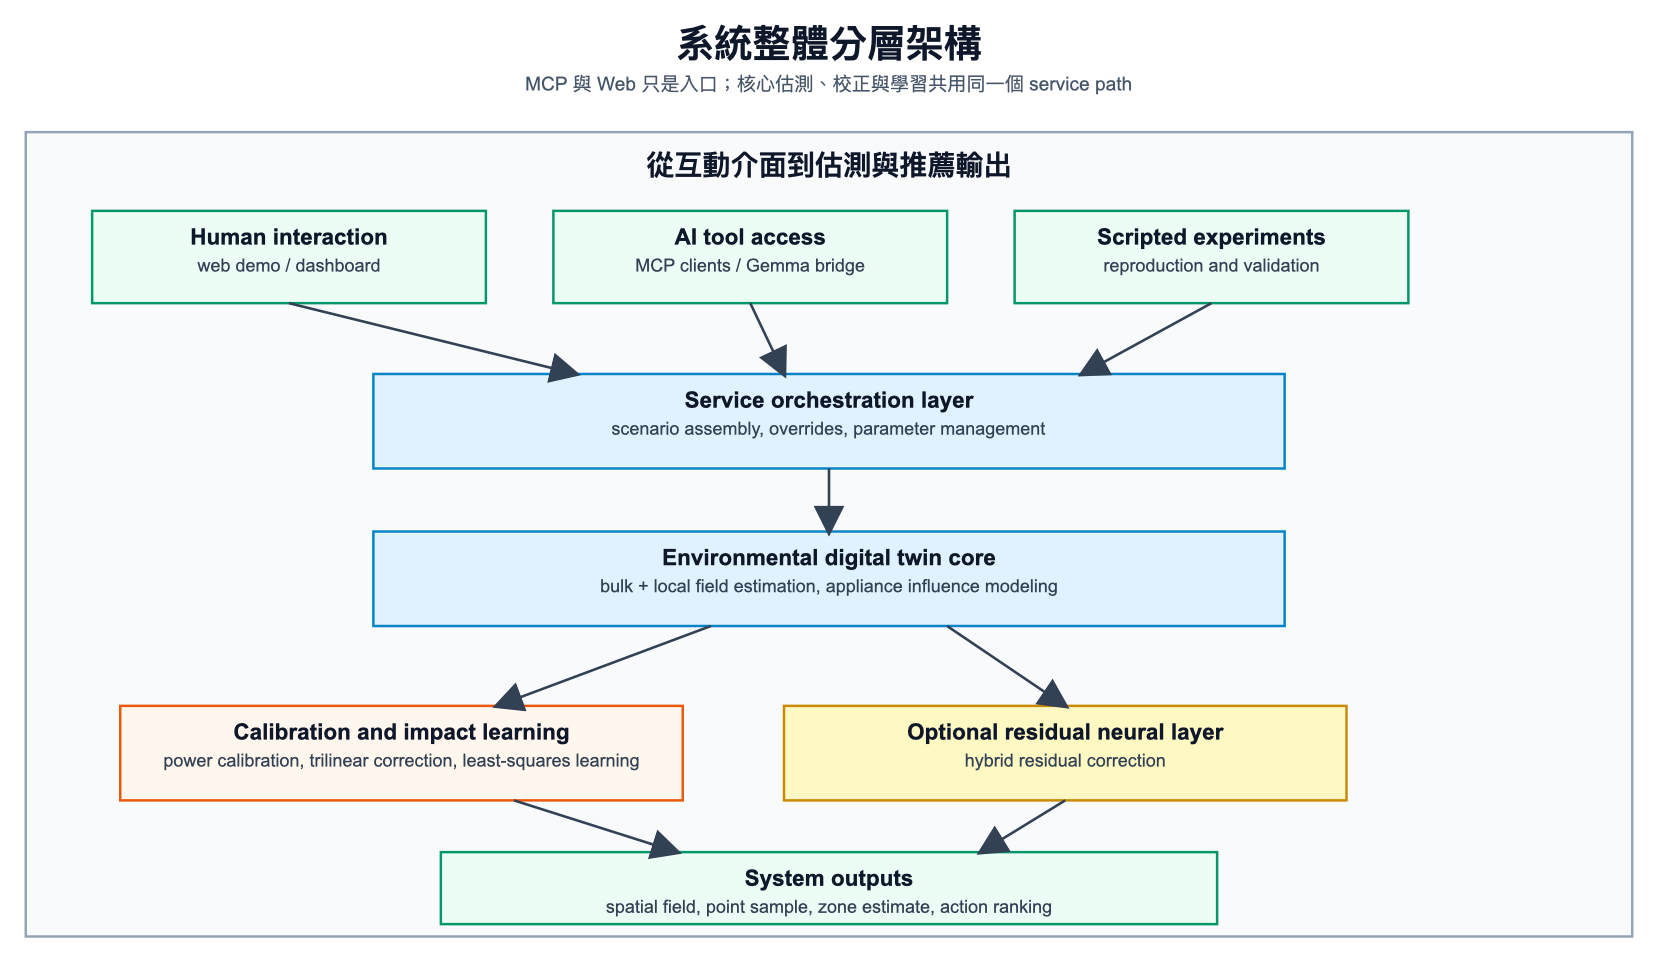
\includegraphics[width=0.83\textwidth]{assets/fig_3_1_overall_architecture.png}
\par\smallskip
{\small 圖 3-1 系統整體分層架構。此圖說明人機互動或 AI 工具呼叫如何經由服務編排層進入環境數位孿生核心、校正與影響學習層，以及 optional residual neural layer，最後輸出空間估測與控制建議。}
\end{figure}

\begin{figure}[htbp]
\centering
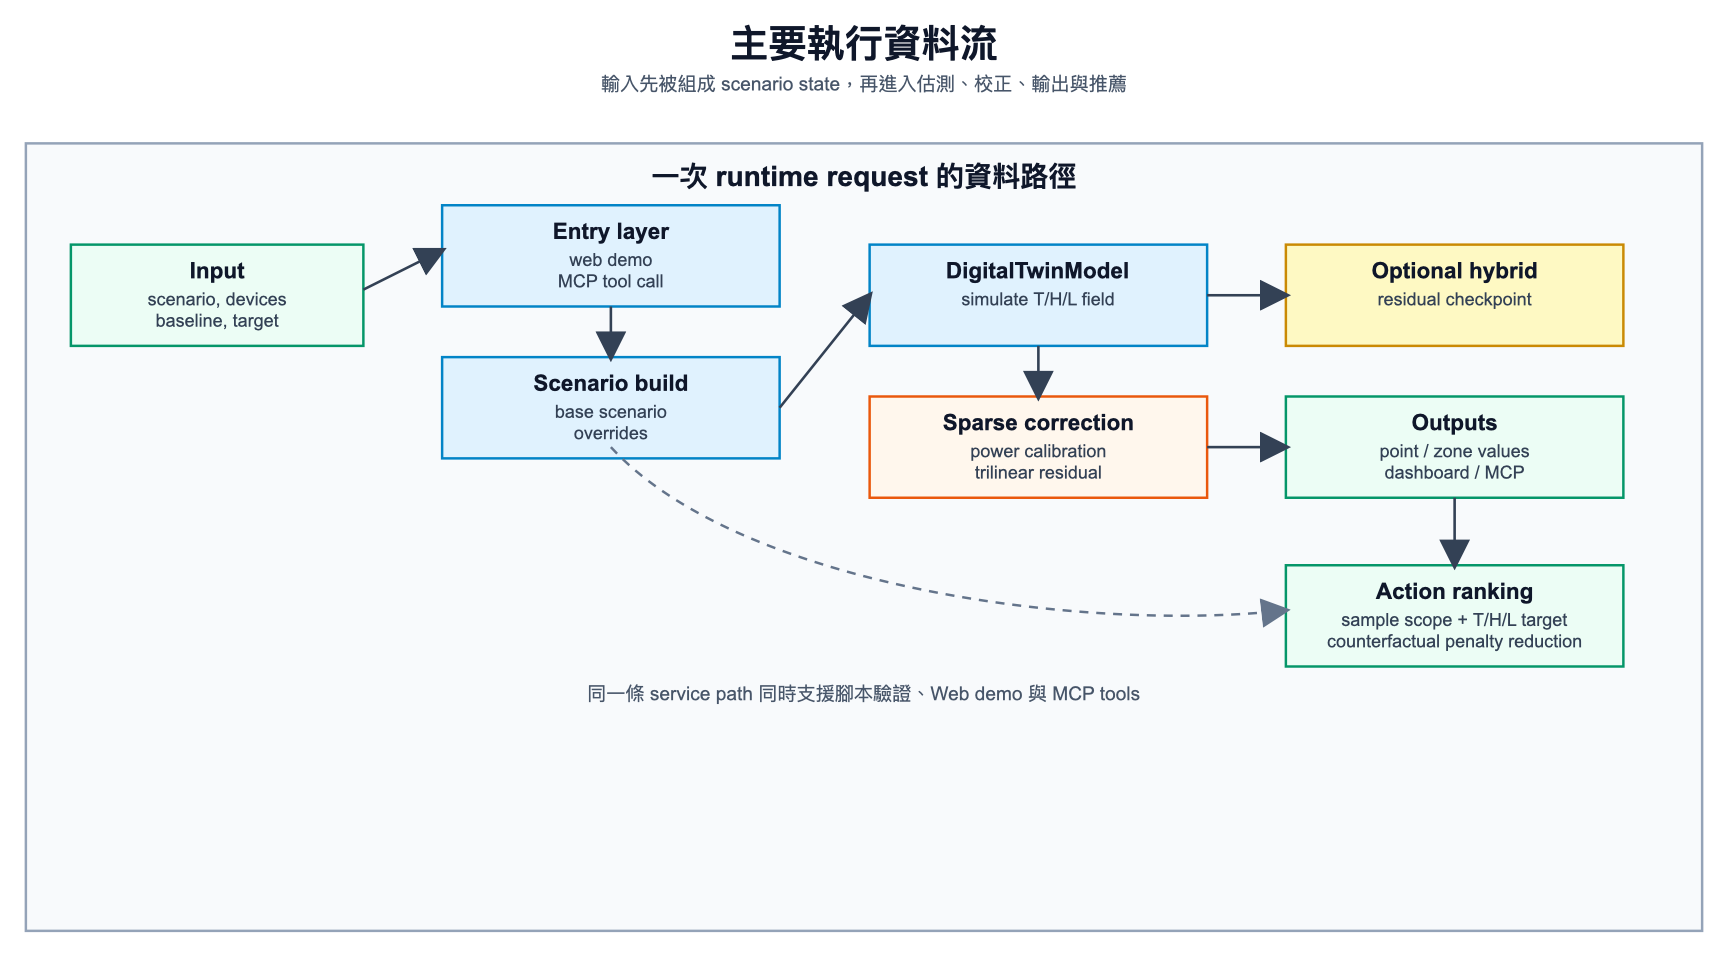
\includegraphics[width=0.90\textwidth]{assets/fig_3_2_execution_flow.png}
\par\smallskip
{\small 圖 3-2 主要執行資料流。此圖對應一次 scenario 評估如何從輸入設定、場估計、校正、到 dashboard 與 MCP 輸出。}
\end{figure}

\subsection*{3.2 房間、區域與感測器設定}

標準房間尺寸設定為寬 6.0 m、長 4.0 m、高 3.0 m。感測器固定於地面四角與天花板四角，共 8 顆節點。每個節點皆假設可量測 temperature、humidity 與 illuminance。區域劃分包含 window\_\allowbreak{}zone、center\_\allowbreak{}zone 與 door\_\allowbreak{}side\_\allowbreak{}zone，用於比較不同空間區域受到設備影響的差異。


\begin{table}[htbp]
\centering
\footnotesize
\begin{tabular}{|p{0.24\textwidth}|p{0.62\textwidth}|}
\hline
\textbf{項目} & \textbf{設定} \\
\hline
房間尺寸 & 6.0 m × 4.0 m × 3.0 m \\
\hline
感測器數量 & 8 顆角落節點 \\
\hline
採樣網格 & 16 × 12 × 6 \\
\hline
三個環境因素 & Temperature, Humidity, Illuminance \\
\hline
主要區域 & window\_\allowbreak{}zone, center\_\allowbreak{}zone, door\_\allowbreak{}side\_\allowbreak{}zone \\
\hline
設備類型 & ac\_\allowbreak{}main, window\_\allowbreak{}main, light\_\allowbreak{}main \\
\hline
\end{tabular}
\end{table}

\begin{figure}[htbp]
\centering
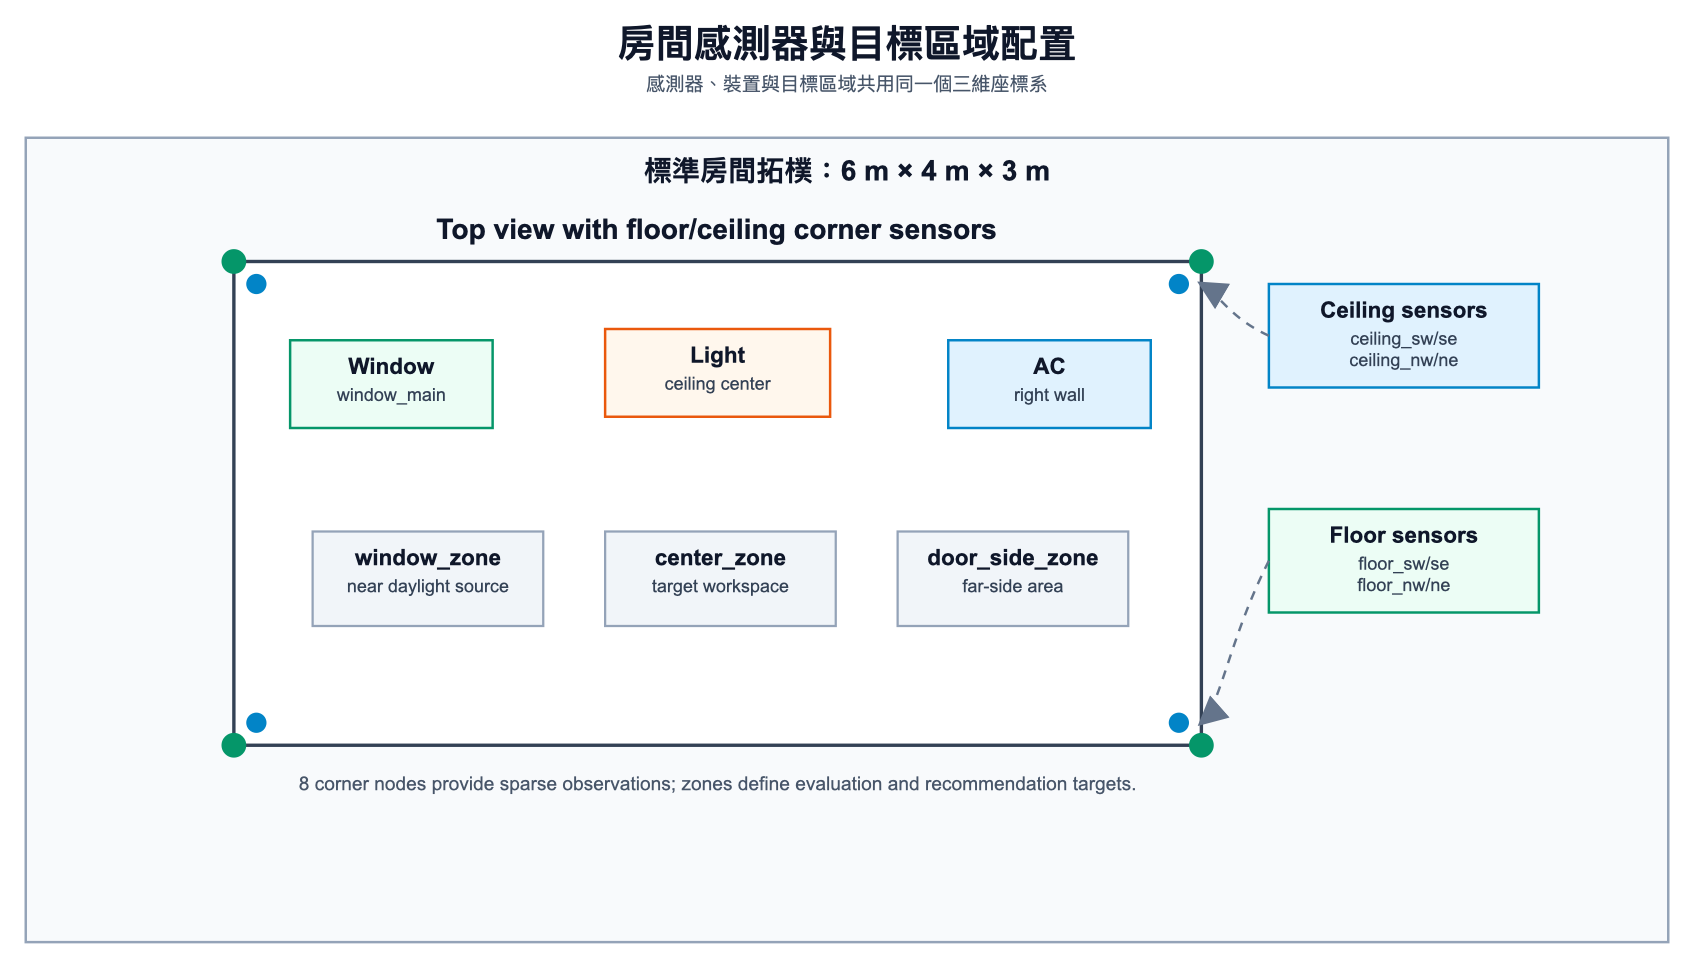
\includegraphics[width=0.90\textwidth]{assets/fig_3_3_room_topology.png}
\par\smallskip
{\small 圖 3-3 房間感測器與目標區域配置。8 顆角落感測器、3 個主要區域與 3 個核心裝置共同構成單房間數位孿生的標準拓樸。}
\end{figure}

\subsection*{3.3 三因子場模型}

本研究將室內狀態定義為三個空間與時間函數：


\[
T(\mathbf{p},t),\quad H(\mathbf{p},t),\quad L(\mathbf{p},t)
\]

任一環境因素 v 的估計場可表示為：


\[
F_v(\mathbf{p},t) = B_v^{\text{bulk}}(t) + B_v^{\text{local}}(\mathbf{p},t) + \sum_j I_{j,v}^{\text{local}}(\mathbf{p},t) + C_v(\mathbf{p})
\]

\begin{itemize}
\item $B_v^{\text{bulk}}$：房間整體平均狀態，描述全室在時間軸上逐漸接近準穩態的平均變化。
\item $B_v^{\text{local}}$：局部背景場，保留簡化垂直分層與空間差異。
\item $I_{j,v}^{\text{local}}$：第 $j$ 個設備對環境因素 $v$ 的局部影響函數。
\item $C_v$：由感測器殘差推估出的校正場。
\end{itemize}

其中 bulk 與 local 的分離是本研究模型的重要改良。若僅使用局部影響場，容易產生冷氣附近很冷，但房間遠端幾乎維持原溫的不合理結果；加入 bulk state 後，模型能同時表示整體房間平均溫濕度的時間響應，以及冷氣出風口、窗邊交換與照明附近的局部差異。此設計也更接近 reduced-order spatial twin 與 zonal or hybrid model 的方法定位 [4][6]。


\subsection*{3.4 設備影響函數}

\begin{itemize}
\item 冷氣：主要造成局部降溫，並帶有弱除濕效果；3D 視覺化中以牆面橫條表示。
\item 窗戶：受外部溫度、外部濕度與日照條件影響，同時改變三個環境因素；3D 視覺化中以牆面矩形表示。
\item 照明：主要提升照度，並產生少量熱效應；3D 視覺化中以點狀標記表示。
\end{itemize}

對照度而言，若只使用窗戶與照明的直接項，再乘上遮蔽衰減，常會低估牆面、地板與家具附近的間接回填亮度。若改用完整 radiosity 或 ray tracing，則需要更細的表面材質、反射模型與幾何資訊，且計算成本明顯提高，與本研究稀疏感測、低成本原型的定位不符。因此本研究僅在 illuminance 路徑加入一個 lightweight single-bounce diffuse reflection 近似：


\[
I^{\text{refl}}(\mathbf{p},t) = \sum_{s} \rho_s \bar{I}_s A_s^{\text{rel}} e^{-\|\mathbf{p}-\mathbf{c}_s\|/\ell_s} \max(0,\,\mathbf{n}_s \cdot \hat{\mathbf{r}}_{s\to p})\, V_s(\mathbf{p})
\]

其中 $s$ 代表 floor、ceiling、四面牆與啟用中的家具表面；$\rho_s$ 為表面反射率；$\bar{I}_s$ 為該表面中心由 direct light 接收到的照度；$A_s^{\text{rel}}$ 為正規化後的面積因子；$\ell_s$ 為衰減長度；$V_s(\mathbf{p})$ 則延用既有遮蔽邏輯。這個公式的目的不是做高保真光學渲染，而是在不引入完整光傳輸模擬的前提下，補足 direct light 對 indirect fill light 的低估。


換言之，本研究對 illuminance 的設計取捨是：保留 direct source、directionality 與 obstruction 的可解釋結構，再另外加上一個單次漫反射近似，使牆、地板、天花板與家具能作為次級發光面回填照度。這樣既能維持與現有影響場模型一致的參數化形式，也比 full radiosity 更適合目前的單房間數位孿生原型。


\subsection*{3.5 感測器校正模型}

模型先預測 8 顆角落感測器位置的三因子值，再與觀測值比較得到殘差。為提高環境估計精度，系統先以最小平方法估計 active device 的 power scale，使設備影響函數更接近觀測資料；接著對每一個環境因素，以 8 參數 trilinear correction 擬合角落殘差：


\[
C(\mathbf{p}) = c_0 + c_1 X + c_2 Y + c_3 Z + c_4 XY + c_5 XZ + c_6 YZ + c_7 XYZ
\]

其中 X、Y、Z 為正規化後的房間座標。相較於一階 affine surface，trilinear correction 可使用 8 個角點支撐 8 個校正係數，除了整體偏移與一階梯度外，也能表示角落之間的交互變化。不過此方法仍無法重建任意高頻局部變化，因此其定位仍是低成本、可解釋的場校正方法。


\begin{figure}[htbp]
\centering
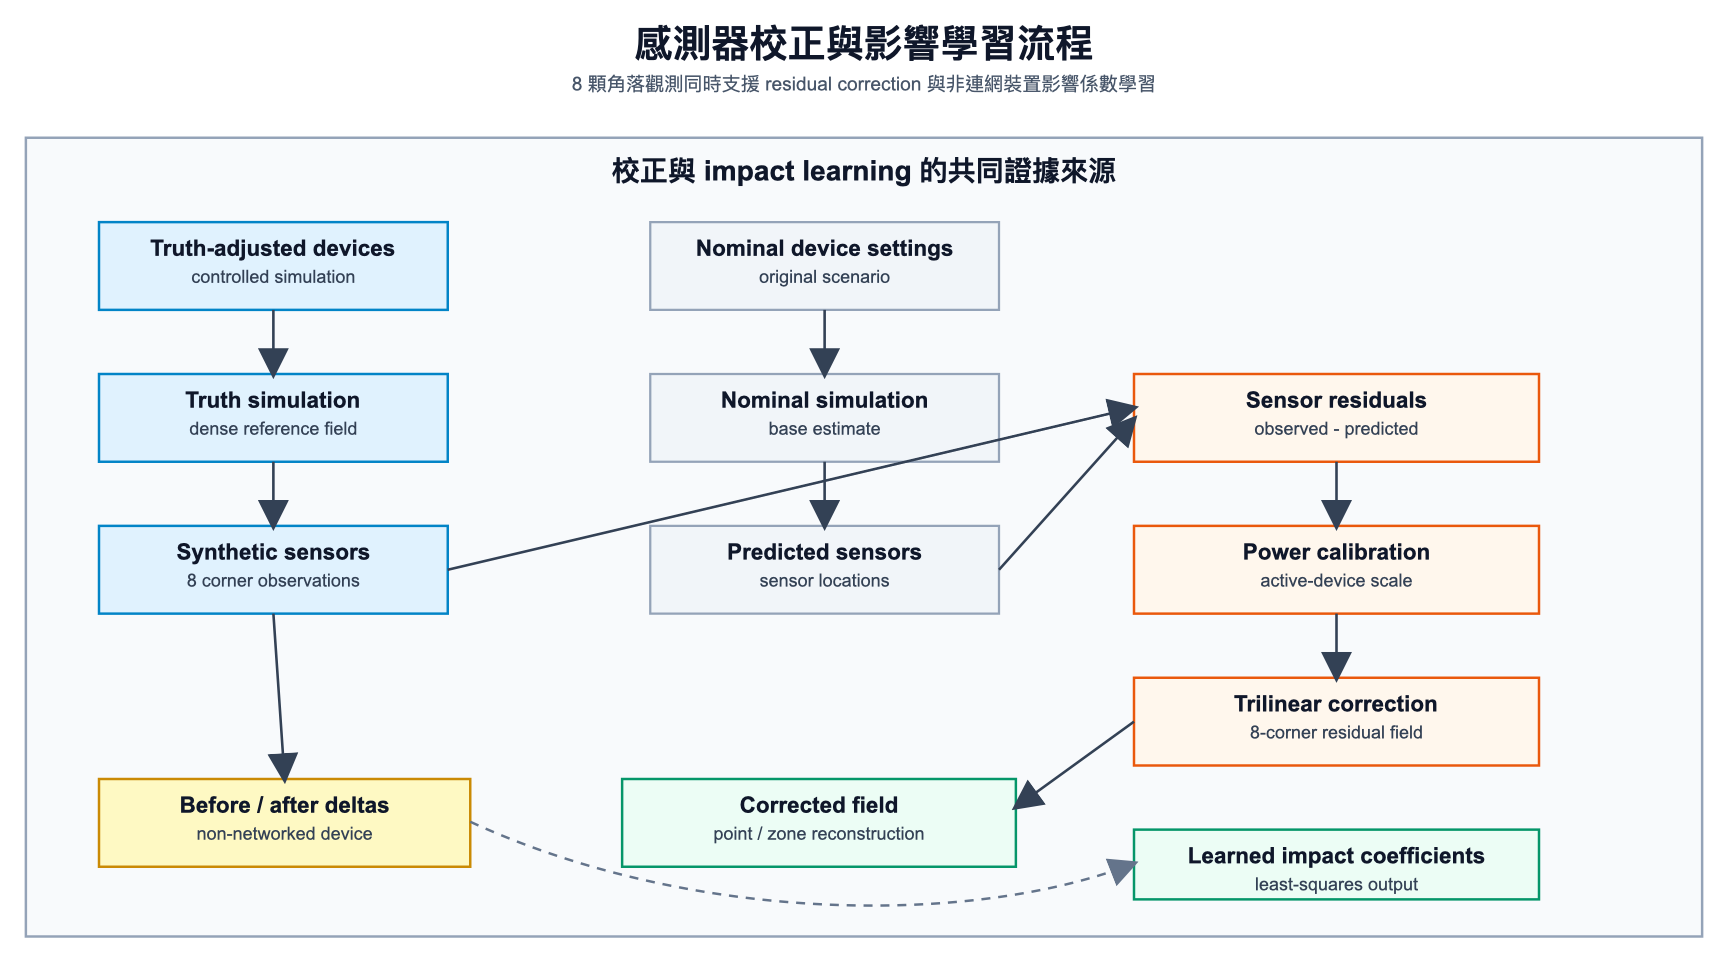
\includegraphics[width=0.83\textwidth]{assets/fig_3_4_sensor_calibration_learning.png}
\par\smallskip
{\small 圖 3-4 感測器校正與影響學習流程。此圖說明真值模擬、角落觀測、設備 power calibration、trilinear residual correction，以及 least-squares impact learning 之間的關係。}
\end{figure}

\subsection*{3.6 非連網裝置影響學習}

對非連網裝置，系統不依賴裝置 API，而是由啟用前後的感測器變化估計影響係數。流程如下：


\begin{lstlisting}[basicstyle=\footnotesize\ttfamily,breaklines=true,columns=flexible]
before sensor observations
-> after sensor observations
-> sensor delta
-> device spatial basis
-> least-squares impact coefficient learning
\end{lstlisting}

\subsection*{3.7 訓練資料組裝流程}

為了讓模型不只停留在手動指定參數，本研究將資料流程拆成原始紀錄層、對齊整併層、樣本建構層與模型訓練層。原始資料至少包含四類：角落感測器時序、裝置事件紀錄、室外環境時序，以及情境描述或額外空間量測。角落感測器時序紀錄 8 顆節點在各時間點的 temperature、humidity 與 illuminance；裝置事件紀錄保存冷氣、窗戶與燈的啟用狀態、模式、設定溫度與開窗比例；室外環境時序提供 outdoor temperature、outdoor humidity 與 sunlight；情境描述則記錄房間尺寸、目標區域、家具配置與採樣設定。


\begin{table}[htbp]
\centering
\footnotesize
\begin{tabular}{|p{0.273\textwidth}|p{0.273\textwidth}|p{0.273\textwidth}|}
\hline
\textbf{資料表} & \textbf{主要欄位} & \textbf{角色} \\
\hline
corner\_\allowbreak{}sensor\_\allowbreak{}timeseries & timestamp, sensor\_\allowbreak{}name, x, y, z, temperature, humidity, illuminance & 提供 8 顆角落感測器觀測值，用於校正、裝置影響學習與真實資料 fine-tune \\
\hline
device\_\allowbreak{}event\_\allowbreak{}log & timestamp, device\_\allowbreak{}name, device\_\allowbreak{}kind, activation, mode, target\_\allowbreak{}temperature, opening\_\allowbreak{}ratio & 還原各時間點裝置狀態，並作為特徵與影響學習依據 \\
\hline
outdoor\_\allowbreak{}environment & timestamp, outdoor\_\allowbreak{}temperature, outdoor\_\allowbreak{}humidity, sunlight\_\allowbreak{}illuminance, daylight\_\allowbreak{}factor & 提供窗戶影響函數與時間條件所需的外部邊界 \\
\hline
scenario\_\allowbreak{}metadata / spatial\_\allowbreak{}probe\_\allowbreak{}ground\_\allowbreak{}truth & 房間尺寸、家具配置、目標區域、額外空間量測 & 定義情境與提供較密集的監督標籤 \\
\hline
\end{tabular}
\end{table}

在資料對齊階段，系統會先以時間戳記為主鍵，將感測器時序、裝置事件與外部環境資料同步到同一時間軸。接著根據房間幾何與裝置配置，將每個時間點的狀態送入主模型，得到 $F_v(\mathbf{p},t)$ 的 physics estimate。若為影響係數學習，則以裝置啟用前後的感測器差值建立 sensor delta；若為 hybrid residual neural network，則進一步在空間採樣點上建立 feature-target 配對。


對於 hybrid residual 訓練，本研究在每個採樣點 $\mathbf{p}_i=(x_i, y_i, z_i)$ 與時間點 $t_i$ 上組合特徵向量：


\[
\boldsymbol{\varphi}_i = [x_i,\, y_i,\, z_i,\, t_i,\, \text{indoor baseline},\, \text{outdoor conditions},\, F_{\text{temp}},\, F_{\text{hum}},\, F_{\text{illum}},\, \text{device activations},\, \text{device powers},\, \text{influence envelopes}]
\]

若採用目前的模擬訓練設定，標籤來自 truth field 與主模型估計值之差：


\[
y_i^v = F_v^{\text{truth}}(\mathbf{p}_i, t_i) - F_v(\mathbf{p}_i, t_i)
\]

其中 v 分別代表 temperature、humidity 與 illuminance。換言之，神經網路不是直接學整個場，而是學主模型剩餘誤差。若未來接入真實資料，則可分成兩種層次：第一種只使用 8 顆角落感測器，將其作為參數校正、裝置影響學習與角落 residual fine-tune 的監督訊號；第二種則在有移動式量測或額外空間探針時，再擴充為更完整的空間 residual 訓練。這樣可避免只憑 8 個角落點就對全室高解析度場做過度宣稱。


在目前的實作中，hybrid residual 訓練可選擇再加入 Fourier low-pass denoising。具體作法是：先針對同一採樣點沿 elapsed time 建立一段短 residual trace，再將該 trace 做 discrete Fourier transform、套用低通遮罩，最後以 inverse transform 還原較平滑的 residual target。根據目前實驗，此做法對 temperature 幾乎不改變結果，對 humidity 有小幅改善，但若直接套用到 illuminance 則會抹去有用的快速變化，因此目前只對 temperature 與 humidity 啟用。


相較於以固定時間窗做積分或區間平均的平滑方式，Fourier low-pass denoising 更適合目前題目。兩者都能降低短時振盪，但時間窗積分本質上屬於時間域中的固定 box filter，若視窗太小則去噪不足，若視窗太大則容易同時模糊瞬態響應與局部轉折，甚至造成較明顯的 lag。相對地，Fourier 低通是直接在頻域中抑制高頻成分，再還原回時間域，因此可以在保留低頻主趨勢的同時，仍然取得對應目前時間點的 denoised residual endpoint。換言之，它不是把時間資訊丟掉，而是在保留時間位置的前提下降低高頻擾動。


整體而言，本研究的訓練資料流程可概括為：原始感測與事件資料先經時間對齊與情境整併，再由主模型產生 physics estimate，最後依任務不同分流為 least-squares impact learning、bulk parameter calibration 或 hybrid residual neural training。此設計的優點在於，即使未來資料來源從模擬切換到真實 ESP32 量測，資料進入訓練流程的接口仍可保持一致。


\subsection*{3.8 Hybrid Residual Neural Network 延伸}

雖然主模型已具有可解釋的 bulk + local field 結構，但在設備交互作用、局部照度分布或窗邊複合邊界條件下，仍可能存在系統性殘差。為此，本研究不以純黑盒神經網路取代主模型，而是加入 hybrid residual neural network 作為第二層修正器：


\[
F_v^{\text{hybrid}}(\mathbf{p},t) = F_v(\mathbf{p},t) + R_v(\mathbf{p},t;\,\boldsymbol{\theta}_v)
\]

其中 $F_v$ 為第三章前述的 reduced-order 主模型，$R_v$ 則由小型多層感知器近似其殘差。訓練目標定義為：


\[
R_v^*(\mathbf{p},t) = F_v^{\text{truth}}(\mathbf{p},t) - F_v(\mathbf{p},t)
\]

其損失函數可表示為：


\[
\mathcal{L}(\boldsymbol{\theta}_v) = \frac{1}{N}\sum_{i=1}^{N}\bigl\|R_v^*(\mathbf{p}_i,t_i) - R_v(\mathbf{p}_i,t_i;\boldsymbol{\theta}_v)\bigr\|^2 + \lambda\|\boldsymbol{\theta}_v\|^2
\]

本研究將座標、時間、室內外環境條件、主模型估計值、設備 activation、設備 power 與 influence envelope 作為輸入特徵，分別為溫度、濕度與照度訓練三個小型殘差網路。若啟用頻域去噪，temperature 與 humidity 會先將 $R_v^*$ 沿短時間軌跡做 Fourier low-pass denoising，再送入 MLP 訓練；illuminance 則保留原始 residual target。此設計的目的在於保留主模型可解釋性，同時以資料驅動方式修正其剩餘誤差。


\subsection*{3.9 控制動作排序}

本研究不做閉環控制，而是對候選控制動作進行排序。系統針對每個候選動作模擬目標區域的三因子值，並依舒適度目標計算改善分數。若房間偏熱，冷氣動作通常獲得較高排序；若照度不足，照明動作通常獲得較高排序。


\clearpage

\section*{第四章 系統實作與服務介面}
\addcontentsline{toc}{section}{第四章 系統實作與服務介面}

\subsection*{4.1 Python 原型}

本研究原型以 Python 實作，核心模組包含 entities、model、scenarios、learning、hybrid\_\allowbreak{}residual、baselines、recommendations、service、mcp\_\allowbreak{}server 與 web\_\allowbreak{}demo。系統採零外部依賴設計，方便在本地環境快速執行與展示。


\begin{table}[htbp]
\centering
\footnotesize
\begin{tabular}{|p{0.24\textwidth}|p{0.62\textwidth}|}
\hline
\textbf{模組} & \textbf{功能} \\
\hline
entities.py & 定義房間、設備、感測器、區域與動作資料結構 \\
\hline
model.py & 建立三因子場、設備影響函數與感測器校正 \\
\hline
scenarios.py & 定義標準情境與窗戶矩陣情境 \\
\hline
learning.py & 由前後感測資料學習非連網裝置影響係數 \\
\hline
hybrid\_\allowbreak{}residual.py & 訓練與套用 hybrid residual neural network \\
\hline
baselines.py & 建立 IDW baseline \\
\hline
service.py & 提供 MCP、Gemma bridge 與 web demo 共用服務介面 \\
\hline
web\_\allowbreak{}demo.py & 提供本地可旋轉 3D web demo \\
\hline
\end{tabular}
\end{table}

\subsection*{4.2 MCP Tools}

本地 MCP server 提供下列 tools：


\begin{itemize}
\item list\_\allowbreak{}scenarios：列出 8 組標準驗證情境。
\item list\_\allowbreak{}window\_\allowbreak{}scenarios：列出 48 組窗戶時段/天氣/季節情境。
\item run\_\allowbreak{}scenario：執行情境並回傳重建誤差與目標區域估計。
\item rank\_\allowbreak{}actions：依目標區域舒適度改善排序候選動作。
\item sample\_\allowbreak{}point：估計指定座標的 temperature、humidity 與 illuminance。
\item compare\_\allowbreak{}baseline：比較本研究模型與 IDW baseline。
\item learn\_\allowbreak{}impacts：由前後感測資料學習非連網裝置影響。
\item run\_\allowbreak{}window\_\allowbreak{}matrix：執行全部 48 組窗戶矩陣模擬。
\item run\_\allowbreak{}window\_\allowbreak{}direct：直接輸入外部溫度、濕度、日照與開窗比例，執行窗戶影響模擬。
\end{itemize}

\subsection*{4.3 Gemma/Ollama Bridge}

本研究以本機 Ollama 上之 Gemma 模型作為語言介面，並以 Python bridge 串接數位孿生服務。實測顯示，本機 Gemma 可透過 Ollama 進行 tool calling；但 MCP 支援本質上來自主機端或 client/runtime 層，而非模型權重本身。因此本研究採用的設計是：由 Gemma 將自然語言請求轉為工具選擇，Python bridge 執行數位孿生服務或 MCP server 所提供的工具，再把工具輸出回送給 Gemma 生成最終回答。這樣的設計比直接宣稱模型原生支援 MCP 更準確，也更符合目前本地 AI agent 的實作方式。


\subsection*{4.4 Web Demo}

Web demo 以 idle 房間背景為基礎，透過 ac\_\allowbreak{}main、window\_\allowbreak{}main 與 light\_\allowbreak{}main checkbox 組合設備狀態，不使用下拉式情境選單。3D 預覽可拖曳旋轉與縮放，並以牆面橫條標示冷氣、牆面矩形標示窗戶、點狀標記表示照明。Metric 亦以勾選式控制切換 temperature、humidity 與 illuminance。左側固定欄位提供 Indoor Baseline 設定，使室內基準溫度、濕度與照度可直接調整；窗戶區則保留季節、天氣與時段 preset，並允許使用者手動覆寫外部溫度與開窗比例。互動式 3D 預覽上方另提供時間軸與播放控制，可觀察系統從啟動到接近準穩態的過程。最新版本的 Web UI 另外提供 estimator toggle，可在主模型與 hybrid residual corrected field 之間切換，並同步更新 target zone、recommendation ranking、baseline comparison、impact panel、3D volume、point sample 與 timeline。


\clearpage

\section*{第五章 模擬案例與結果分析}
\addcontentsline{toc}{section}{第五章 模擬案例與結果分析}

\subsection*{5.1 標準情境設定}

本研究建立 8 組標準情境，包含無設備作用、僅冷氣、僅開窗、僅照明、冷氣與窗戶、窗戶與照明、冷氣與照明，以及三者同時作用。每組情境均輸出場重建誤差、區域平均值、感測器校正效果、IDW baseline 比較、非連網裝置影響學習與推薦排序。


\begin{figure}[htbp]
\centering
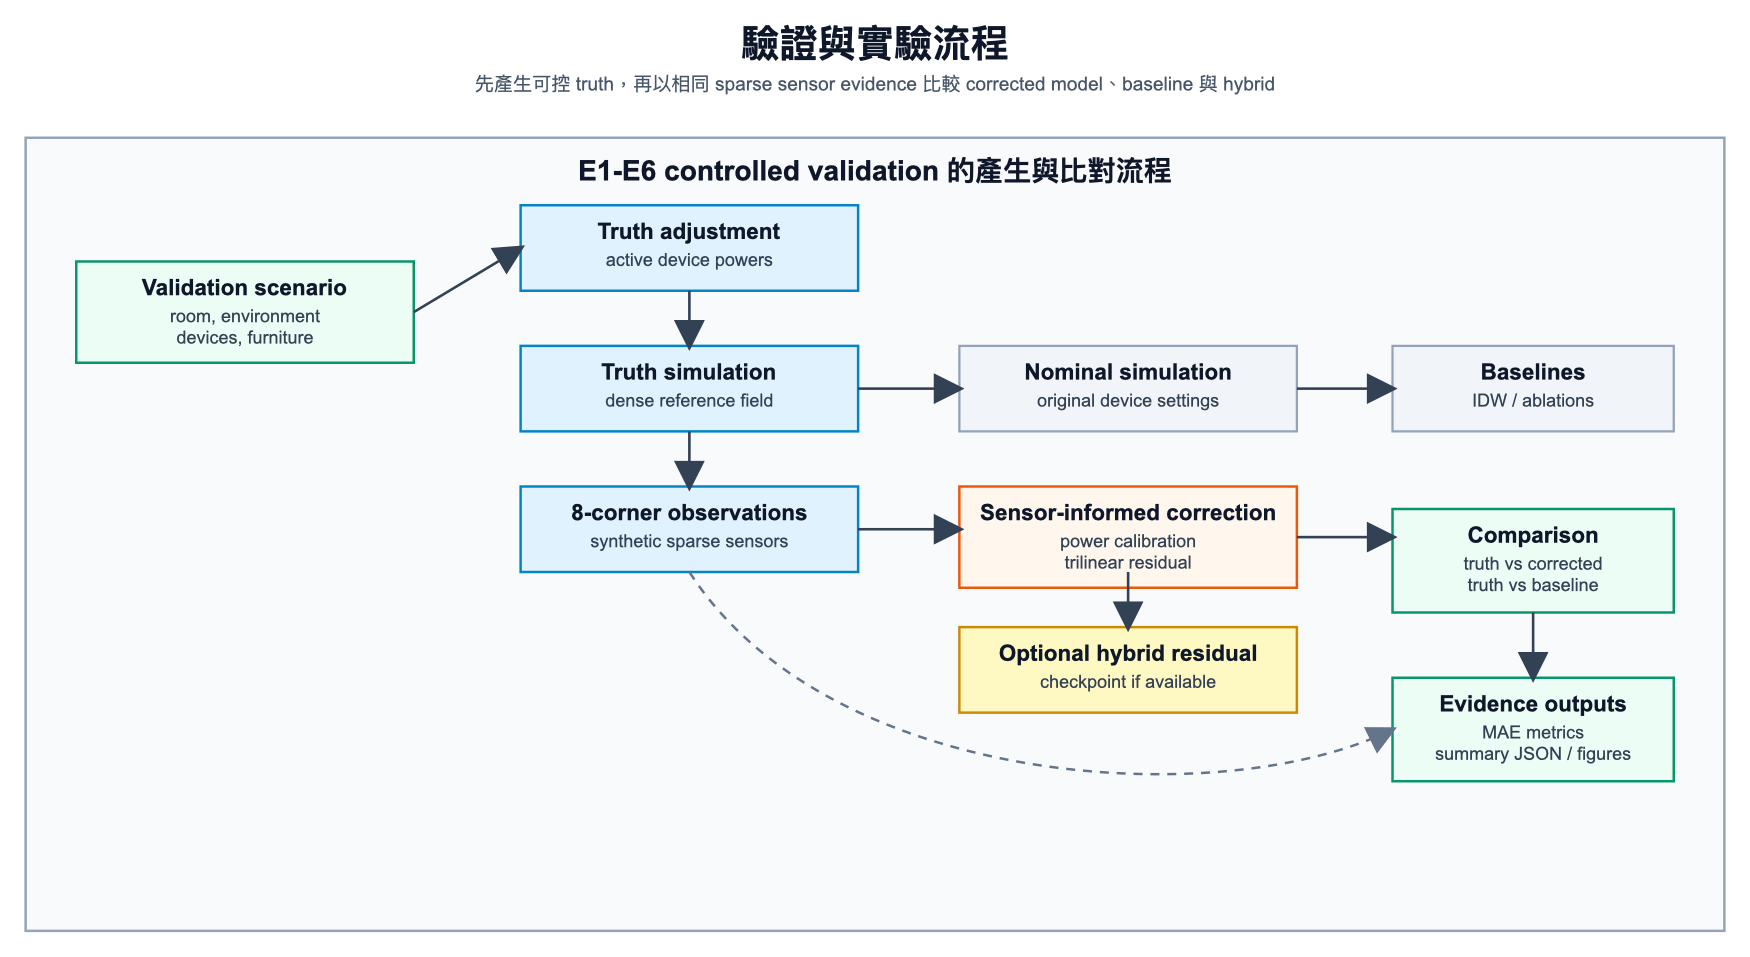
\includegraphics[width=0.83\textwidth]{assets/fig_5_1_validation_flow.png}
\par\smallskip
{\small 圖 5-1 驗證與實驗流程。此圖說明標準情境如何經由 truth adjustment、合成觀測、校正估測、baseline 比較與輸出摘要，形成第五章的實驗結果。}
\end{figure}

表 5-1 標準情境結果摘要


\begin{table}[htbp]
\centering
\footnotesize
\begin{tabular}{|p{0.164\textwidth}|p{0.164\textwidth}|p{0.164\textwidth}|p{0.164\textwidth}|p{0.164\textwidth}|}
\hline
\textbf{情境} & \textbf{中央溫度} & \textbf{中央濕度} & \textbf{中央照度} & \textbf{最佳推薦} \\
\hline
idle & 28.84 & 67.60 & 90.00 & ac\_\allowbreak{}and\_\allowbreak{}light \\
\hline
ac\_\allowbreak{}only & 25.56 & 65.75 & 90.00 & turn\_\allowbreak{}on\_\allowbreak{}light \\
\hline
window\_\allowbreak{}only & 29.51 & 68.42 & 214.60 & ac\_\allowbreak{}and\_\allowbreak{}light \\
\hline
light\_\allowbreak{}only & 29.11 & 67.60 & 452.99 & turn\_\allowbreak{}on\_\allowbreak{}ac \\
\hline
all\_\allowbreak{}active & 26.39 & 66.34 & 478.82 & turn\_\allowbreak{}on\_\allowbreak{}ac \\
\hline
\end{tabular}
\end{table}

\subsection*{5.2 場重建誤差}

本研究採用平均絕對誤差（Mean Absolute Error, MAE）作為主要精度指標，定義如下，其中 ŷᵢ 為模型在第 i 個網格點的預測值，yᵢ 為對應的模擬基準值，n 為評估點總數。MAE 直接反映預測值與基準值之間的平均偏差幅度，數值愈低代表場重建愈準確，且因不進行平方放大，對少數離群點較不敏感，適合作為室內場重建的評估基準。


\[
\text{MAE} = \frac{1}{n}\sum_{i=1}^{n}\left|\hat{y}_i - y_i\right|
\]

8 組標準情境中，平均溫度 MAE 為 0.0474，平均濕度 MAE 為 0.1764，平均照度 MAE 為 2.1288。照度 MAE 仍高於溫度與濕度，主要原因是照度場受燈具位置、窗戶日照、遮蔽與方向性影響較大，且數值尺度遠高於溫度與濕度。相較於前一版只使用 direct source + obstruction 的照度路徑，加入 single-bounce diffuse reflection 後，平均照度 MAE 由 2.1616 降至 2.1288，最大照度 MAE 亦由 2.7090 降至 2.6633。


這表示新增的反射公式確實補足了牆面、地板、天花板與家具造成的間接回填亮度，使非直射區域不再被系統性低估。另一方面，溫度與濕度指標幾乎沒有變化，也說明這組公式主要作用在預期的 illuminance 路徑，而沒有不必要地擾動其他兩個環境因素。


\begin{figure}[htbp]
\centering
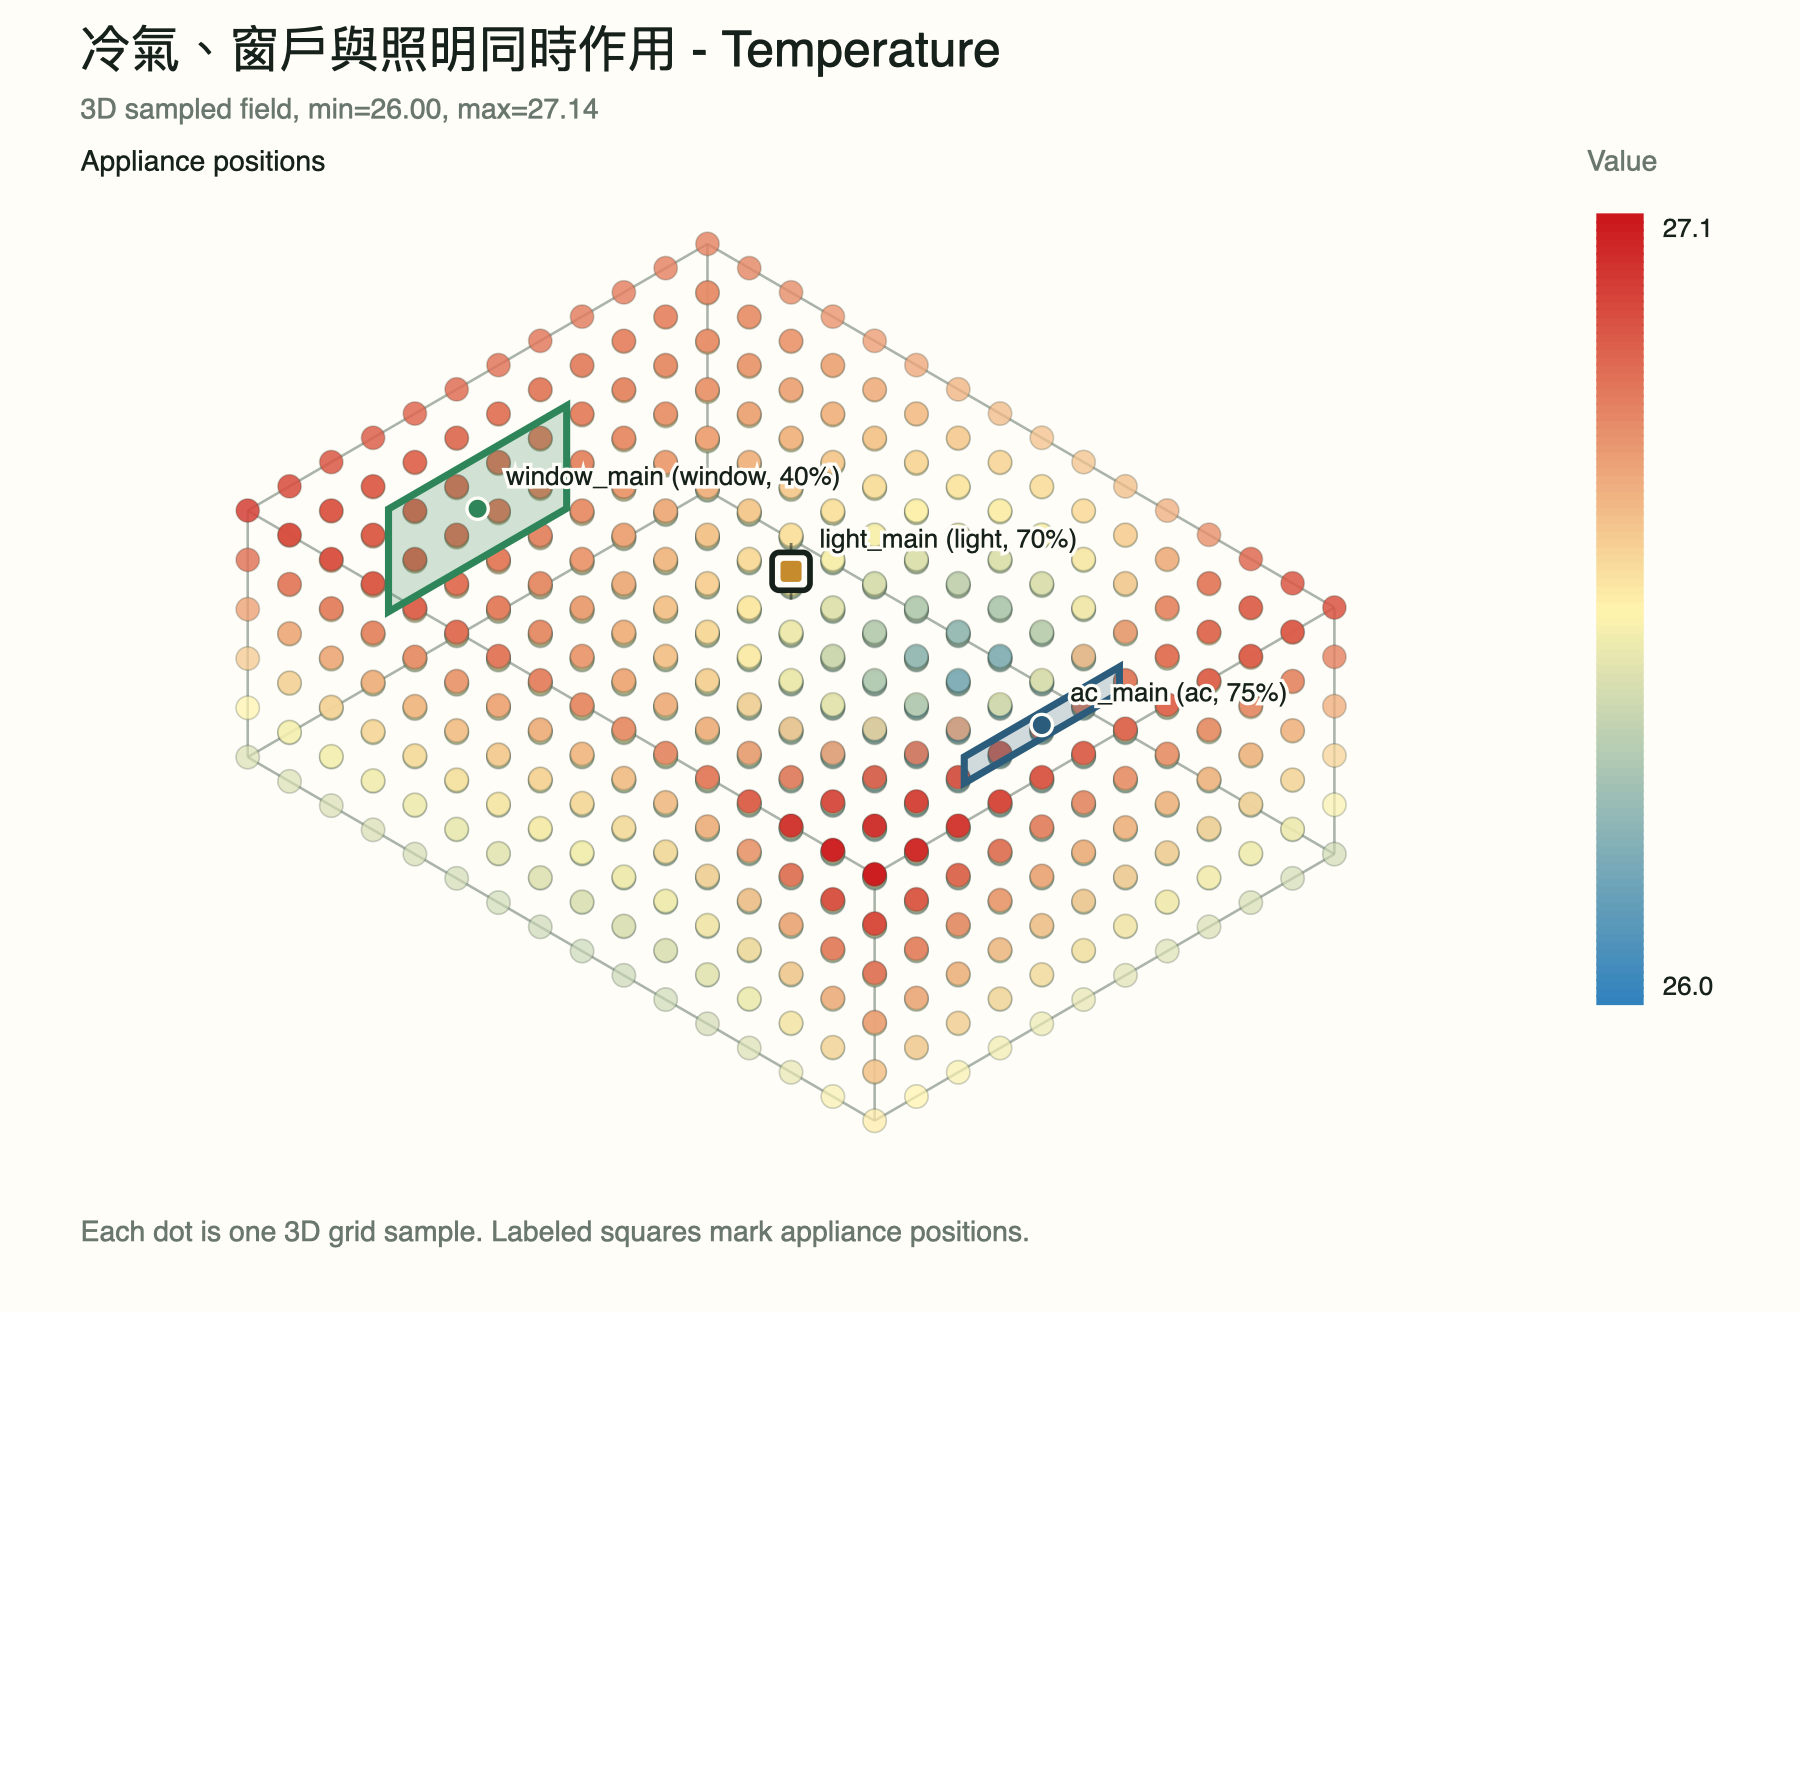
\includegraphics[width=0.83\textwidth]{assets/fig_5_2_all_active_temp_3d.png}
\par\smallskip
{\small 圖 5-2 三裝置同時作用（all\textbackslash{}\_\allowbreak{}active）之溫度場 3D 點雲視圖。每點為一個 16×12×6 網格樣本，顏色由藍綠（低溫）至橙紅（高溫）映射溫度分布。冷氣區域明顯偏藍，靠窗與靠燈區域則居溫度中高端。}
\end{figure}

\begin{figure}[htbp]
\centering
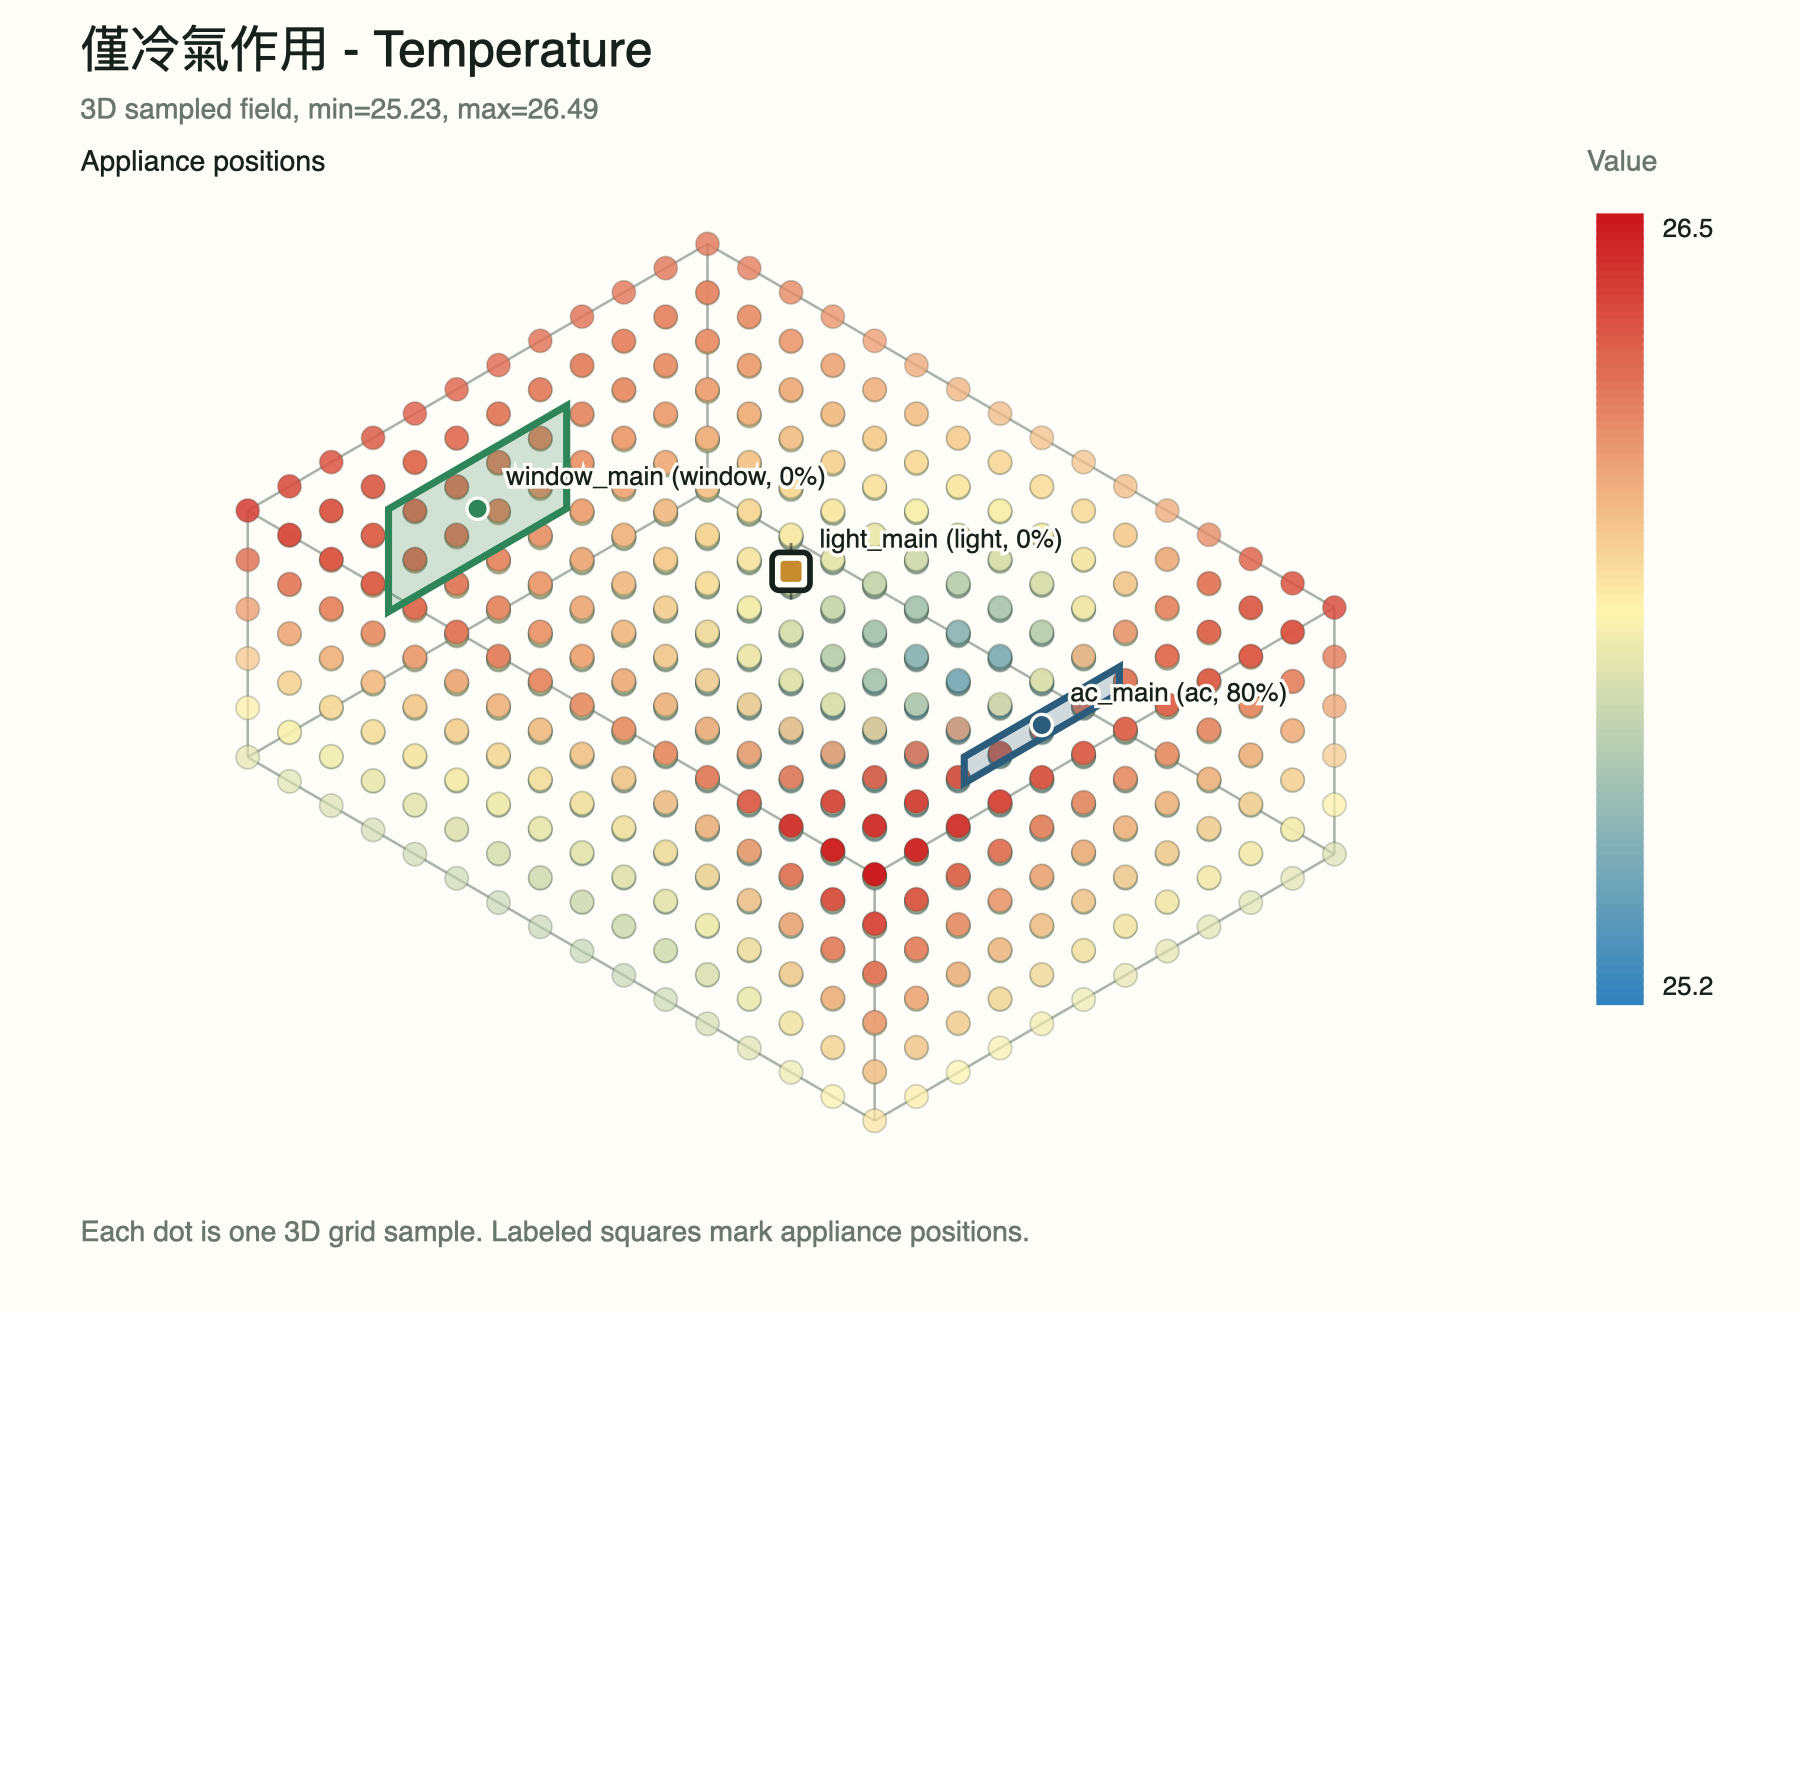
\includegraphics[width=0.83\textwidth]{assets/fig_5_3_ac_only_temp_3d.png}
\par\smallskip
{\small 圖 5-3 僅冷氣作用（ac\textbackslash{}\_\allowbreak{}only）之溫度場 3D 點雲視圖。冷氣氣流影響區域（後牆靠左側）溫度明顯下降，距冷氣較遠的靠窗區域溫度相對較高，展示 bulk + local field 模型對全室平均與局部梯度的同時建模能力。}
\end{figure}

\begin{figure}[htbp]
\centering
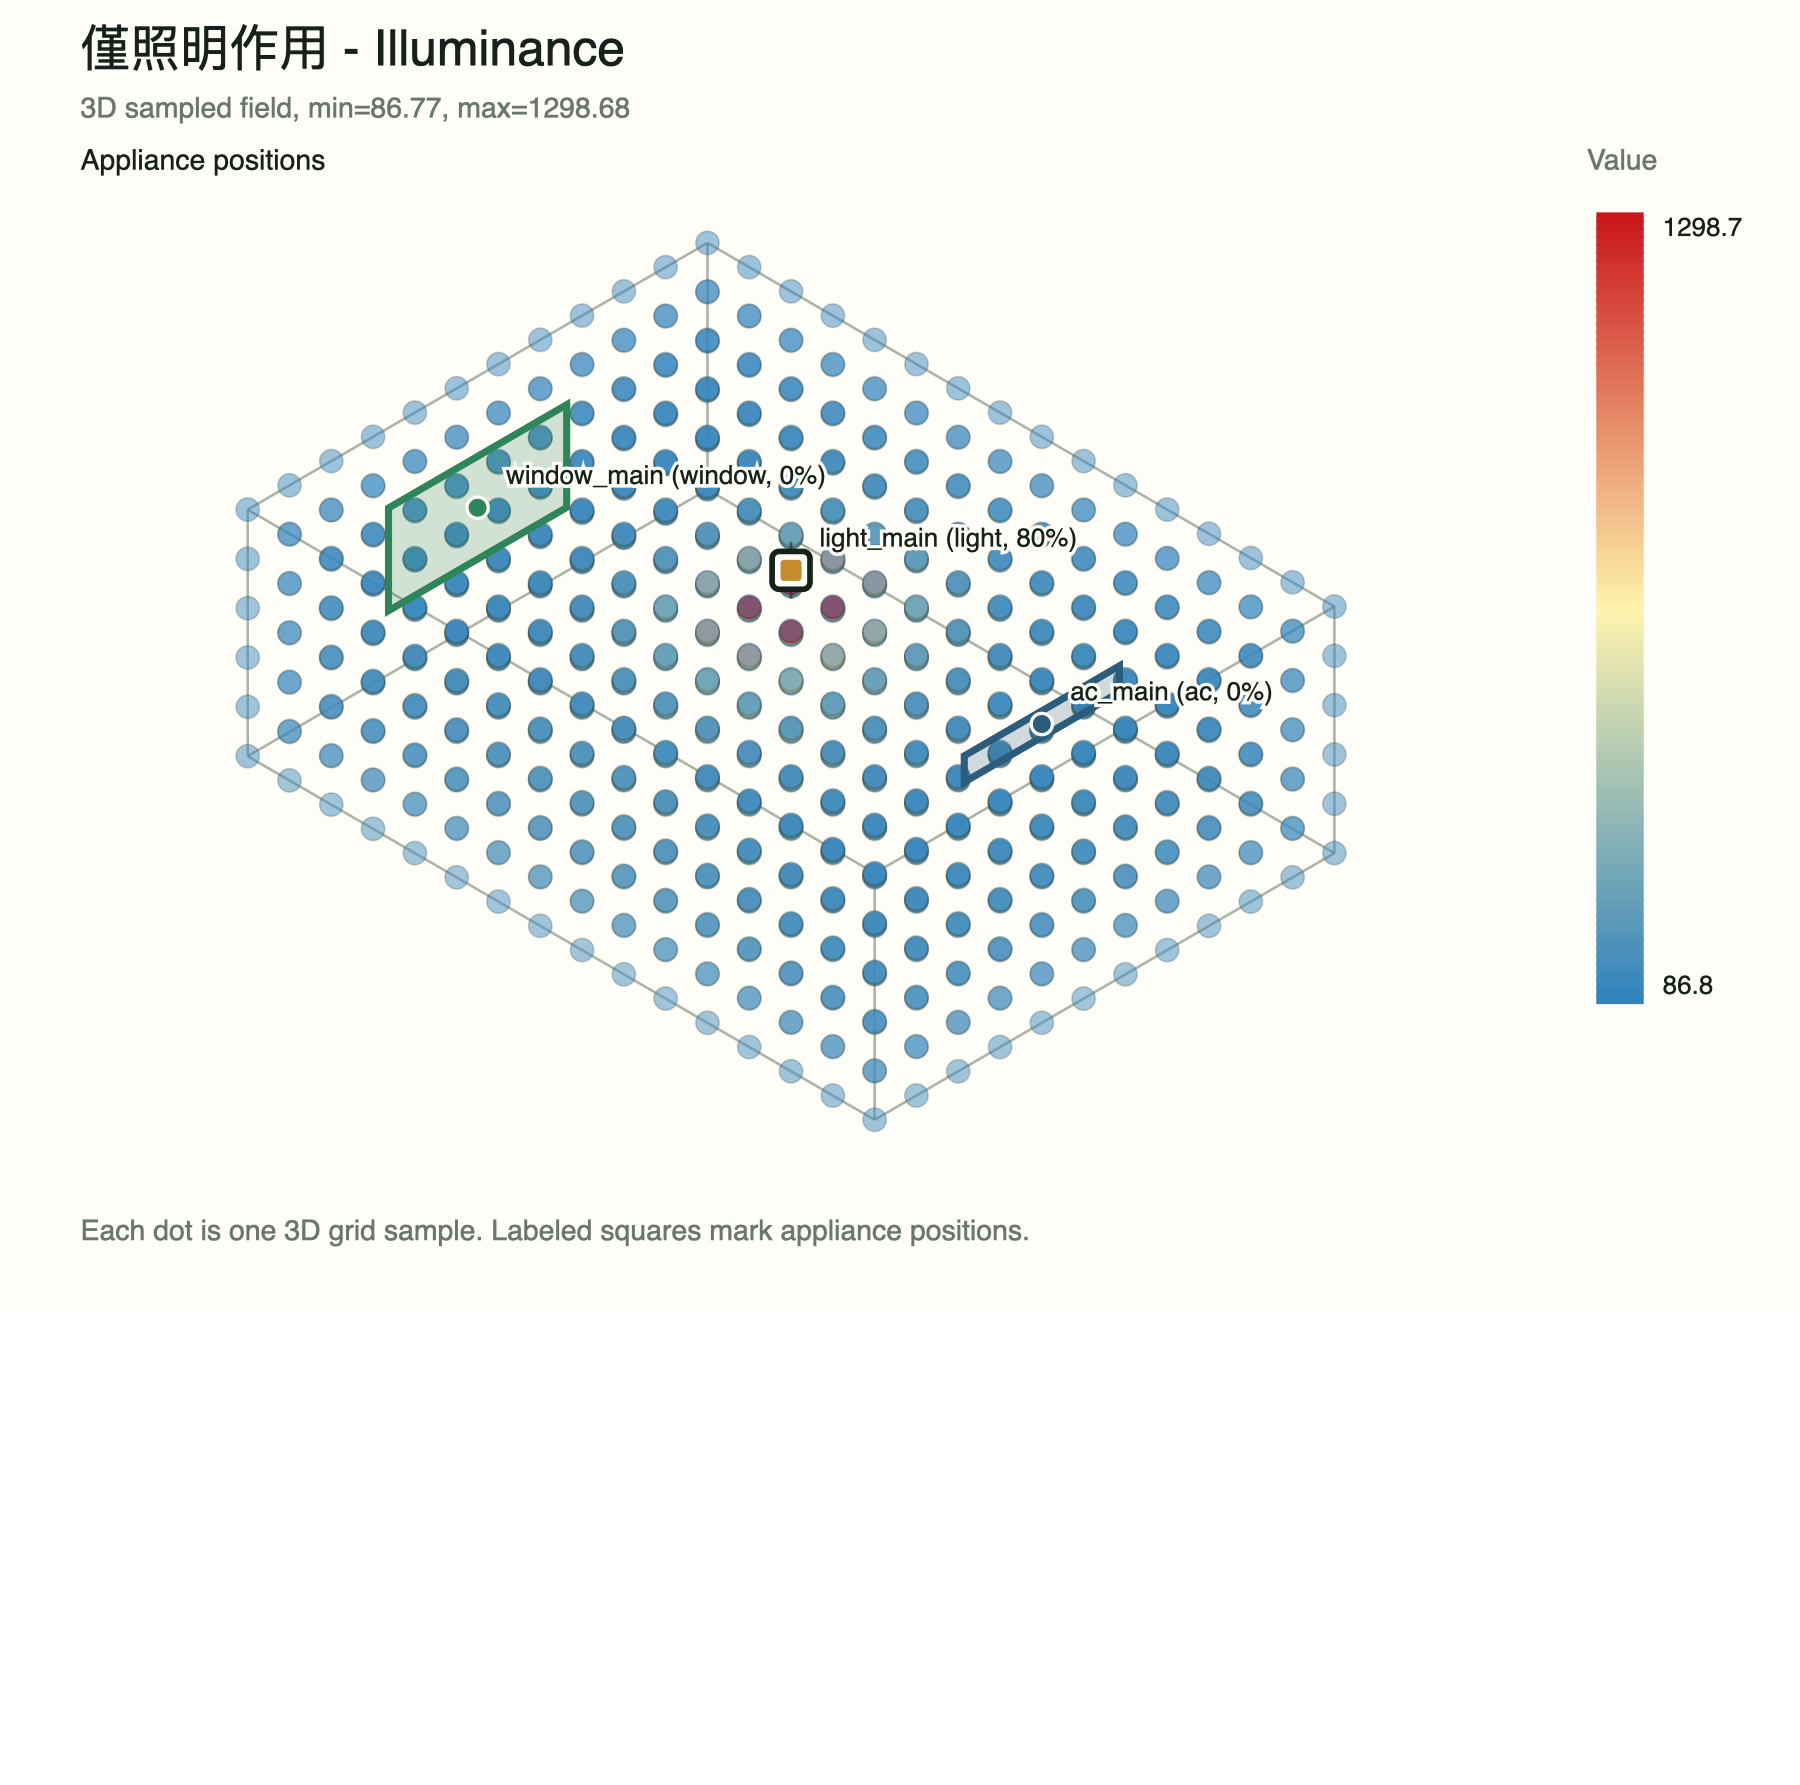
\includegraphics[width=0.83\textwidth]{assets/fig_5_4_light_only_illum_3d.png}
\par\smallskip
{\small 圖 5-4 僅燈具作用（light\textbackslash{}\_\allowbreak{}only）之照度場 3D 點雲視圖。燈具正下方的測點照度最高（黃橙色），底層四角與遠端則由間接反射賦予少量回填亮度，顏色實現正確的照度衰減樣態。}
\end{figure}

\subsection*{5.3 IDW Baseline 比較}

IDW（Inverse Distance Weighting，反距離加權插值）是最基本的空間插值法：給定 8 顆角落感測器的量測值，對任一查詢點以距離的倒數為權重加權平均。此方法不需要任何關於設備位置或物理模型的知識，僅依賴量測點的空間分布進行推算。本節以 IDW 作為零成本 baseline，驗證本研究模型加入設備影響函數、power scale 校準與 trilinear residual correction 後的實質改善幅度。


表 5-2 列出 8 組情境下，IDW 與本研究模型（base model）的 field MAE 及改善比例。


\begin{table}[htbp]
\centering
\footnotesize
\begin{tabular}{|p{0.164\textwidth}|p{0.164\textwidth}|p{0.164\textwidth}|p{0.164\textwidth}|p{0.164\textwidth}|}
\hline
\textbf{情境} & \textbf{因子} & \textbf{本研究 MAE} & \textbf{IDW MAE} & \textbf{改善 (\%)} \\
\hline
idle & 溫度 & 0.0470 & 0.1242 & 62.2\% \\
\hline
idle & 濕度 & 0.1762 & 0.4656 & 62.2\% \\
\hline
idle & 照度 & 1.7625 & 1.3210 & −33.4\% ▲ \\
\hline
ac\textbackslash{}\_\allowbreak{}only & 溫度 & 0.0481 & 0.2536 & 81.0\% \\
\hline
ac\textbackslash{}\_\allowbreak{}only & 照度 & 1.7625 & 1.3210 & −33.4\% ▲ \\
\hline
window\textbackslash{}\_\allowbreak{}only & 照度 & 2.3024 & 58.7291 & 96.1\% \\
\hline
light\textbackslash{}\_\allowbreak{}only & 溫度 & 0.0470 & 0.1306 & 64.0\% \\
\hline
light\textbackslash{}\_\allowbreak{}only & 照度 & 2.6633 & 129.9798 & 97.9\% \\
\hline
window\textbackslash{}\_\allowbreak{}light & 照度 & 1.9913 & 167.9708 & 98.8\% \\
\hline
ac\textbackslash{}\_\allowbreak{}light & 照度 & 2.5770 & 121.8574 & 97.9\% \\
\hline
all\textbackslash{}\_\allowbreak{}active & 溫度 & 0.0477 & 0.1883 & 74.7\% \\
\hline
all\textbackslash{}\_\allowbreak{}active & 照度 & 1.9957 & 147.2720 & 98.6\% \\
\hline
\end{tabular}
\end{table}

結果說明如下。在溫度與濕度方面，所有情境的改善率均達 61–81\%，原因是本研究模型加入冷氣對全室與局部溫濕度的設備影響函數，使有設備的情境（ac\textbackslash{}\_\allowbreak{}only、ac\textbackslash{}\_\allowbreak{}window、ac\textbackslash{}\_\allowbreak{}light、all\textbackslash{}\_\allowbreak{}active）能正確描述冷氣區域的降溫效果，而純 IDW 因僅依靠角落感測值做全場推算，對冷氣作用區域估計不準。


在照度方面，有光源（窗戶或燈具）的情境改善幅度極大（96–99\%），原因是照度具有強烈的點源衰減特性：燈具正下方的照度極高，角落卻很低，IDW 用角落感測值插值中央會嚴重低估；而本研究模型使用直接照度公式加 single-bounce diffuse reflection，能正確重建燈具中心的高照度峰值。對照地，idle 與 ac\textbackslash{}\_\allowbreak{}only（無窗無燈）的照度改善為負，這是預期現象：在無主動光源情境下，照度全場平坦，IDW 插值本身即有合理表現，本研究模型的設備驅動照度項此時不起作用，反而略高於 IDW 的平坦估計。此結果反映本研究照度建模設計的目標：在有光源時大幅提升精度，而非在無光源情境下多此一舉。


值得注意的是，本研究目前的照度估計完全依賴物理模型推算（設備位置、功率、反射係數），並未使用任何實測照度感測器回饋。若系統部署時，角落感測器本身即具備照度量測能力（例如採用光照感測元件的多合一環境感測器），則可將實測角落照度值引入 trilinear residual correction，使模型的照度殘差直接對齊真實量測，從根本上消除物理假設帶來的系統性偏差。換言之，本研究現有的照度誤差並非方法的根本限制，而是感測器配置選擇的結果，一旦取得真實光照量測資料，即可透過既有的 residual correction 管線加以修正，實現更高精度的照度場重建。


\subsection*{5.4 非連網裝置影響學習}

在 ac\_\allowbreak{}only 情境中，模型學得冷氣對 temperature 的係數為負，對 humidity 的係數亦為負，對 illuminance 則接近零，符合冷氣降溫與弱除濕的模型假設。在 light\_\allowbreak{}only 情境中，照明主要提升 illuminance，並帶來少量正向熱效應。這些結果顯示，即使裝置本身不回報狀態，仍可由環境感測變化估計其影響方向與相對強度。


\subsection*{5.5 窗戶時段、天氣、季節矩陣與直接輸入}

本研究新增 48 組窗戶矩陣情境，組合 4 個時段、3 種天氣與 4 個季節。此矩陣可作為外部環境變數敏感度分析，用於說明窗戶在不同外部條件下對靠窗區與中心區的溫度、濕度與照度影響。


除列舉矩陣外，系統亦支援窗戶 direct input 模式。使用者可直接提供外部溫度、外部濕度、外部日照照度、開窗比例，以及可選的室內基準溫濕度。此模式適合接入即時天氣資料、手動量測資料或使用者指定條件，不必先將外部條件離散化為季節、天氣與時段分類。


\begin{table}[htbp]
\centering
\footnotesize
\begin{tabular}{|p{0.164\textwidth}|p{0.164\textwidth}|p{0.164\textwidth}|p{0.164\textwidth}|p{0.164\textwidth}|}
\hline
\textbf{情境} & \textbf{外部溫度} & \textbf{外部濕度} & \textbf{外部日照} & \textbf{窗戶區照度} \\
\hline
window\_\allowbreak{}summer\_\allowbreak{}sunny\_\allowbreak{}noon & 37.0 & 71.0 & 36000.0 & 243.7090 \\
\hline
window\_\allowbreak{}winter\_\allowbreak{}rainy\_\allowbreak{}night & 11.0 & 78.0 & 15.2 & 68.9740 \\
\hline
window\_\allowbreak{}spring\_\allowbreak{}cloudy\_\allowbreak{}morning & 21.5 & 70.0 & 5005.0 & 93.2172 \\
\hline
\end{tabular}
\end{table}

\subsection*{5.6 Hybrid Residual Neural Network 結果}

在目前預設的 held-out 測試設定下，hybrid residual neural network 以 6 個情境作為訓練資料，並以 light\textbackslash{}\_\allowbreak{}only 與 all\textbackslash{}\_\allowbreak{}active 作為測試情境（與 5.2 節的 8 組全集平均為不同子集）。若對 temperature 與 humidity residual trace 啟用 Fourier low-pass denoising，並保留 illuminance 原始 residual，則 hybrid residual correction 套用於主模型輸出後，field MAE 可由 temperature 0.0474、humidity 0.1764、illuminance 2.3295，分別降至 0.0026、0.0040 與 0.1752。對應改善比例約為溫度 94.51\%、濕度 97.73\% 與照度 92.48\%。


若與加入反射近似前的 direct-only 照度路徑相比，held-out illuminance 的主模型 MAE 由 2.3727 降至 2.3295，而 hybrid 後的 illuminance MAE 由 0.2357 進一步降至 0.1752。這表示較乾淨的 base optical approximation 可先降低結構性照度偏差，再讓 residual network 更集中地學習剩餘誤差；而頻域低通則較適合作為慢變 thermal / humidity residual 的前處理，而非對所有環境因子一體適用。不過此結果仍建立於模擬資料與既定情境分割下，未來仍需以真實量測資料重新訓練與驗證。


\subsection*{5.7 公開資料集 Task-Aligned Benchmark 結果}

為驗證模型在非合成資料上的外部可比性，本研究以 SML2010 與 CU-BEMS 兩個公開資料集執行 task-aligned benchmark，並以 MAE、RMSE 與 Pearson Correlation 三項指標進行評估。MAE 衡量平均絕對誤差，RMSE 對尖峰偏差更敏感，Correlation 則反映模型是否能正確追蹤時序趨勢，三者共同提供較完整的評估視角。預測目標為下一個 15 分鐘或 60 分鐘時步的感測值，比較對象為 persistence（以上一時步值作預測）與 linear regression 兩個 baseline。


表 5-4 列出 SML2010 benchmark 各任務三項指標的完整對比。


\begin{table}[htbp]
\centering
\footnotesize
\begin{tabular}{|p{0.117\textwidth}|p{0.117\textwidth}|p{0.117\textwidth}|p{0.117\textwidth}|p{0.117\textwidth}|p{0.117\textwidth}|p{0.117\textwidth}|}
\hline
\textbf{任務} & \textbf{視窗} & \textbf{目標} & \textbf{指標} & \textbf{Persistence} & \textbf{Linear Reg} & \textbf{本研究} \\
\hline
S1 照度 & 15min & dining\_\allowbreak{}illuminance & MAE & 3.418 & 4.023 & 5.346 \\
\hline
S1 照度 & 15min & dining\_\allowbreak{}illuminance & RMSE & 8.074 & 8.194 & 9.986 \\
\hline
S1 照度 & 15min & dining\_\allowbreak{}illuminance & Corr & 0.963 & 0.966 & 0.957 \\
\hline
S2 溫度 & 15min & dining\_\allowbreak{}temperature & MAE & 0.118 & 0.043 & 0.073 \\
\hline
S2 溫度 & 15min & dining\_\allowbreak{}temperature & RMSE & 0.135 & 0.056 & 0.089 \\
\hline
S2 溫度 & 15min & dining\_\allowbreak{}temperature & Corr & 0.999 & 1.000 & 0.999 \\
\hline
S2 濕度 & 15min & dining\_\allowbreak{}humidity & MAE & 0.198 & 0.209 & 0.832 \\
\hline
S2 濕度 & 15min & dining\_\allowbreak{}humidity & RMSE & 0.304 & 0.316 & 1.026 \\
\hline
S2 濕度 & 15min & dining\_\allowbreak{}humidity & Corr & 0.998 & 0.998 & 0.988 \\
\hline
S3 複合溫度 & 15min & dining\_\allowbreak{}temperature & MAE & 0.233 & 0.093 & 0.071 \\
\hline
S3 複合溫度 & 15min & dining\_\allowbreak{}temperature & RMSE & 0.283 & 0.115 & 0.089 \\
\hline
S3 複合溫度 & 15min & dining\_\allowbreak{}temperature & Corr & 0.000 & 0.909 & 0.950 \\
\hline
S3 複合濕度 & 15min & dining\_\allowbreak{}humidity & MAE & 0.386 & 0.393 & 0.335 \\
\hline
S3 複合濕度 & 15min & dining\_\allowbreak{}humidity & RMSE & 0.595 & 0.574 & 0.475 \\
\hline
S3 複合濕度 & 15min & dining\_\allowbreak{}humidity & Corr & 0.000 & 0.337 & 0.612 \\
\hline
S3 複合照度 & 15min & dining\_\allowbreak{}illuminance & MAE & 8.473 & 9.813 & 9.437 \\
\hline
S3 複合照度 & 15min & dining\_\allowbreak{}illuminance & RMSE & 14.449 & 13.623 & 13.552 \\
\hline
S3 複合照度 & 15min & dining\_\allowbreak{}illuminance & Corr & 0.000 & 0.526 & 0.366 \\
\hline
S3 複合溫度 & 60min & dining\_\allowbreak{}temperature & MAE & 0.563 & 0.212 & 0.190 \\
\hline
S3 複合溫度 & 60min & dining\_\allowbreak{}temperature & RMSE & 0.693 & 0.256 & 0.243 \\
\hline
S3 複合溫度 & 60min & dining\_\allowbreak{}temperature & Corr & 0.000 & 0.906 & 0.937 \\
\hline
S3 複合濕度 & 60min & dining\_\allowbreak{}humidity & MAE & 0.889 & 0.809 & 0.759 \\
\hline
S3 複合濕度 & 60min & dining\_\allowbreak{}humidity & RMSE & 1.281 & 1.155 & 1.059 \\
\hline
S3 複合濕度 & 60min & dining\_\allowbreak{}humidity & Corr & 0.000 & 0.434 & 0.569 \\
\hline
S3 複合照度 & 60min & dining\_\allowbreak{}illuminance & MAE & 15.209 & 17.170 & 14.460 \\
\hline
S3 複合照度 & 60min & dining\_\allowbreak{}illuminance & RMSE & 21.931 & 22.763 & 19.344 \\
\hline
S3 複合照度 & 60min & dining\_\allowbreak{}illuminance & Corr & 0.000 & 0.715 & 0.472 \\
\hline
\end{tabular}
\end{table}

表 5-5 列出 CU-BEMS benchmark 各任務三項指標的完整對比。


\begin{table}[htbp]
\centering
\footnotesize
\begin{tabular}{|p{0.117\textwidth}|p{0.117\textwidth}|p{0.117\textwidth}|p{0.117\textwidth}|p{0.117\textwidth}|p{0.117\textwidth}|p{0.117\textwidth}|}
\hline
\textbf{任務} & \textbf{視窗} & \textbf{目標} & \textbf{指標} & \textbf{Persistence} & \textbf{Linear Reg} & \textbf{本研究} \\
\hline
C1 溫濕度 & 15min & temperature & MAE & 0.262 & 0.288 & 0.282 \\
\hline
C1 溫濕度 & 15min & temperature & RMSE & 0.574 & 0.534 & 0.530 \\
\hline
C1 溫濕度 & 15min & temperature & Corr & 0.980 & 0.983 & 0.983 \\
\hline
C1 溫濕度 & 15min & humidity & MAE & 0.713 & 0.778 & 0.756 \\
\hline
C1 溫濕度 & 15min & humidity & RMSE & 1.468 & 1.452 & 1.457 \\
\hline
C1 溫濕度 & 15min & humidity & Corr & 0.978 & 0.979 & 0.979 \\
\hline
C2 照度 & 15min & illuminance & MAE & 1.363 & 1.794 & 7.700 \\
\hline
C2 照度 & 15min & illuminance & RMSE & 6.344 & 6.264 & 11.938 \\
\hline
C2 照度 & 15min & illuminance & Corr & 0.962 & 0.963 & 0.864 \\
\hline
C3 複合溫度 & 15min & temperature & MAE & 0.571 & 0.692 & 0.626 \\
\hline
C3 複合溫度 & 15min & temperature & RMSE & 1.301 & 1.124 & 1.153 \\
\hline
C3 複合溫度 & 15min & temperature & Corr & 0.000 & 0.503 & 0.479 \\
\hline
C3 複合照度 & 60min & illuminance & MAE & 4.509 & 7.093 & 5.728 \\
\hline
C3 複合照度 & 60min & illuminance & RMSE & 12.507 & 12.162 & 12.105 \\
\hline
C3 複合照度 & 60min & illuminance & Corr & 0.000 & 0.263 & 0.228 \\
\hline
C2 照度 & 60min & illuminance & MAE & 4.012 & 5.646 & 9.566 \\
\hline
C2 照度 & 60min & illuminance & RMSE & 12.065 & 11.575 & 14.234 \\
\hline
C2 照度 & 60min & illuminance & Corr & 0.864 & 0.866 & 0.792 \\
\hline
\end{tabular}
\end{table}

\subsubsection*{5.7.1 優勢分析}

第一項優勢是複合任務的趨勢追蹤能力。在 S3 與 C3 等複合任務中，persistence 的 Correlation 值全為 0.000，原因是這些任務包含裝置切換或外部條件突變，使前一時步值完全失去預測能力。相較之下，本研究模型在 S3 15min dining\_\allowbreak{}temperature 的 Correlation 達 0.950，S3 15min dining\_\allowbreak{}humidity 達 0.612，S3 60min dining\_\allowbreak{}temperature 達 0.937，均為三者最高。這說明物理結構與設備影響函數提供的先驗資訊，在環境條件快速變化時比純時序延續有更強的趨勢預測能力。


第二項優勢是長視窗溫度任務的 MAE 與 RMSE。以 S3 dining\_\allowbreak{}temperature 為例，在 60 分鐘預測視窗下，本研究的 MAE 為 0.190、RMSE 為 0.243，均為三者最低；相較之下 persistence 為 0.563 與 0.693，linear regression 為 0.212 與 0.256。這說明當預測視窗拉長時，納入設備狀態與外部條件的結構性估計比單純延續前一時步更穩定。


第三項優勢是複合任務的 RMSE 表現。以 S3 60min dining\_\allowbreak{}illuminance 為例，本研究的 RMSE 為 19.344，低於 persistence 的 21.931 與 linear regression 的 22.763。RMSE 對離群誤差的放大效應更敏感，這表示本研究模型在極端照度事件的重建上較其他方法更為穩定。


\subsubsection*{5.7.2 劣勢分析}

最明顯的劣勢出現在短視窗純照度任務。SML2010 S1 15min dining\_\allowbreak{}illuminance 的 MAE 為 5.346，高於 persistence 的 3.418 與 linear regression 的 4.023；Correlation 為 0.957，略低於另外兩者的 0.963 與 0.966。CU-BEMS C2 15min illuminance 的差距更大，MAE 7.700 對比 persistence 1.363，RMSE 11.938 對比 persistence 6.344。主要原因是短視窗照度的最佳預測策略接近 persistence（照度在 15 分鐘內變化緩慢），而本研究在對應時段的日照估計引入了額外誤差，反而不如直接沿用上一時步值。


第二個劣勢是 SML2010 濕度的系統性高估。S2 15min dining\_\allowbreak{}humidity 的 MAE 為 0.832，遠高於 persistence 的 0.198 與 linear regression 的 0.209。這反映本研究的濕度特徵對齊方式與 SML2010 的量測尺度存在系統性偏差，即模型濕度估計值的基準點偏移，而非隨機誤差。此問題在 S3 複合任務中得到部分改善（S3 dining\_\allowbreak{}humidity MAE 0.335，接近 persistence 0.386），推測是複合任務的外氣濕度特徵提供了更多修正訊號。


第三個劣勢是 CU-BEMS C2 純照度任務在 60 分鐘視窗下的表現。MAE 9.566 遠高於 persistence 4.012，RMSE 14.234 也高於 persistence 12.065，且 Correlation 0.792 低於 persistence 0.864。CU-BEMS 的照度量測來自多區商辦建築，其照度動態特性（日光、遮蔽、人工照明切換）與本研究單房間物理假設差距較大，使得照度估計誤差在長視窗下難以收斂。


綜合三項指標，本研究的設計優勢集中在「複合任務、長視窗、裝置切換情境下的趨勢追蹤與誤差穩定性」，弱點則在「短視窗純照度預測」與「與本研究感測拓樸不匹配之外部資料集的濕度估計」。這與本研究的設計定位一致：模型的核心目的是空間場估計與裝置影響學習，而非最小化單一時序預測指標。


需要特別說明的是，task-aligned benchmark 採用的是「下一時步預測」框架（15min 或 60min 視窗），而本研究的核心使用情境並非短視窗自回歸預測，而是在設備達到準穩態後的空間場估計。實際應用中，使用者先啟動冷氣或開窗，系統再估計若干分鐘後整個房間的三因子空間分布，並據此輸出控制動作推薦。此類穩態導向估計不依賴前一時步值作為主要訊號，而是依賴設備配置、外部環境條件與物理影響函數。因此，persistence 在短視窗下的優勢屬於不同任務假設的產物，並不代表本研究模型在其實際設計目標上的劣勢。本研究進行 task-aligned benchmark 的目的，是為了在共同可比的框架下提供外部資料集的相對定位，而非宣稱本研究的主要評估對象是次步預測誤差。


\subsection*{5.8 研究過程與實作挑戰}

本研究在實作過程中有三個直接影響最終模型設計的問題。第一，初期若僅使用 local field 疊加設備作用，會出現冷氣附近快速降溫、房間遠端卻幾乎維持原溫的不合理結果，因此後續必須加入 bulk state 描述全室平均狀態的時間收斂。第二，若只以 8 顆角落感測器直接監督整個 3D 場，則黑盒神經網路雖可能把角落點擬合得很好，但對室內中央、窗邊與家具後方的場仍缺乏足夠監督，因此本研究把神經網路限制在 residual correction 層，而不是直接取代主模型。第三，公開資料集與本研究情境在幾何、裝置標記與感測器拓樸上通常不一致，因此必須採用 task-aligned benchmark，不能直接把所有實驗都搬到同一公開資料集上比較。


這些困難也說明本研究的設計取捨不是任意拼接，而是由實作過程逐步收斂而來：bulk + local field 負責處理全室與局部差異，single-bounce diffuse reflection 負責補足 direct lighting 對間接回填亮度的低估，trilinear correction 負責利用有限角落感測器修正低階偏差，least-squares impact learning 負責從設備前後差異學習非連網裝置影響，hybrid residual neural network 則只處理主模型尚未吸收的系統性誤差。


\subsection*{5.9 可旋轉 3D 展示}

Web demo 提供可旋轉 3D 預覽，使使用者可直接觀察三因子點雲、房間框線與設備幾何位置。冷氣以牆面橫條表示，窗戶以牆面矩形表示，照明以點狀標記表示。圖 5-5 至 5-7 為靜態輸出之三因子場 3D 點雲，展示三種代表情境：三裝置全開、單獨窗戶、單獨燈具。此展示有助於口試或公開展示時說明模型如何從設備位置與環境場估計區域影響。


\begin{figure}[htbp]
\centering
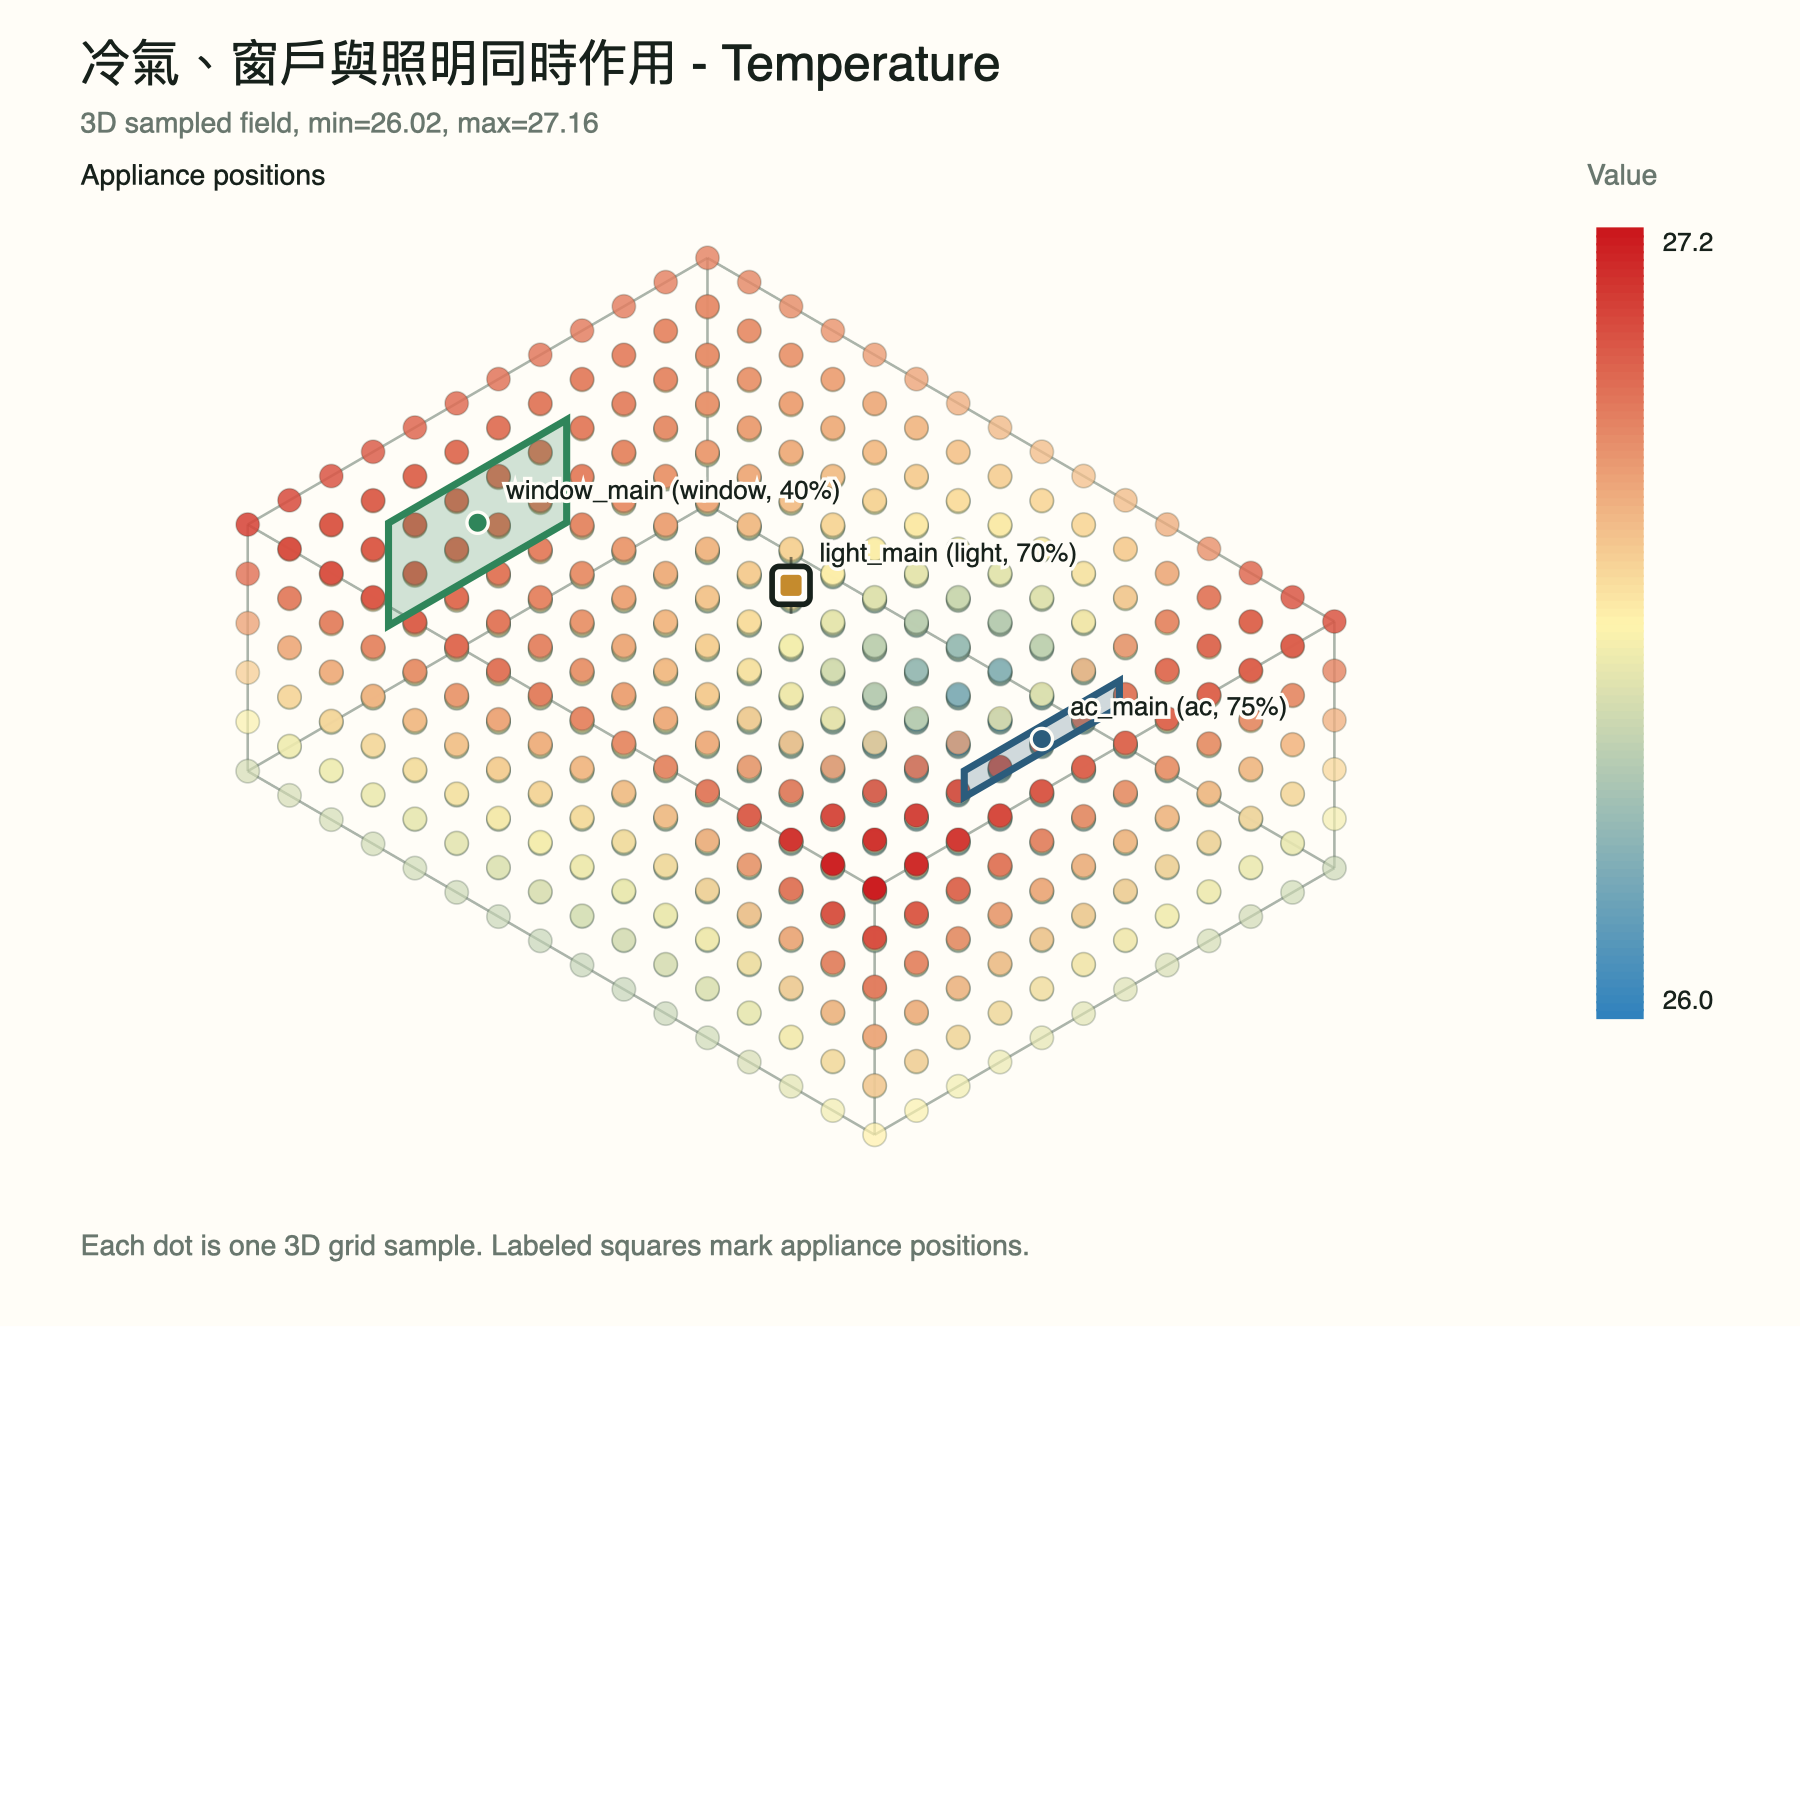
\includegraphics[width=0.83\textwidth]{assets/fig_5_5_all_active_temp_3d.png}
\par\smallskip
{\small 圖 5-5 三裝置同時作用（all\textbackslash{}\_\allowbreak{}active）溫度場 3D 點雲。顏色由藍綠至橙紅對映 26.02–27.16 °C 範圍；設備位置用帶邊框的標記表示。}
\end{figure}

\begin{figure}[htbp]
\centering
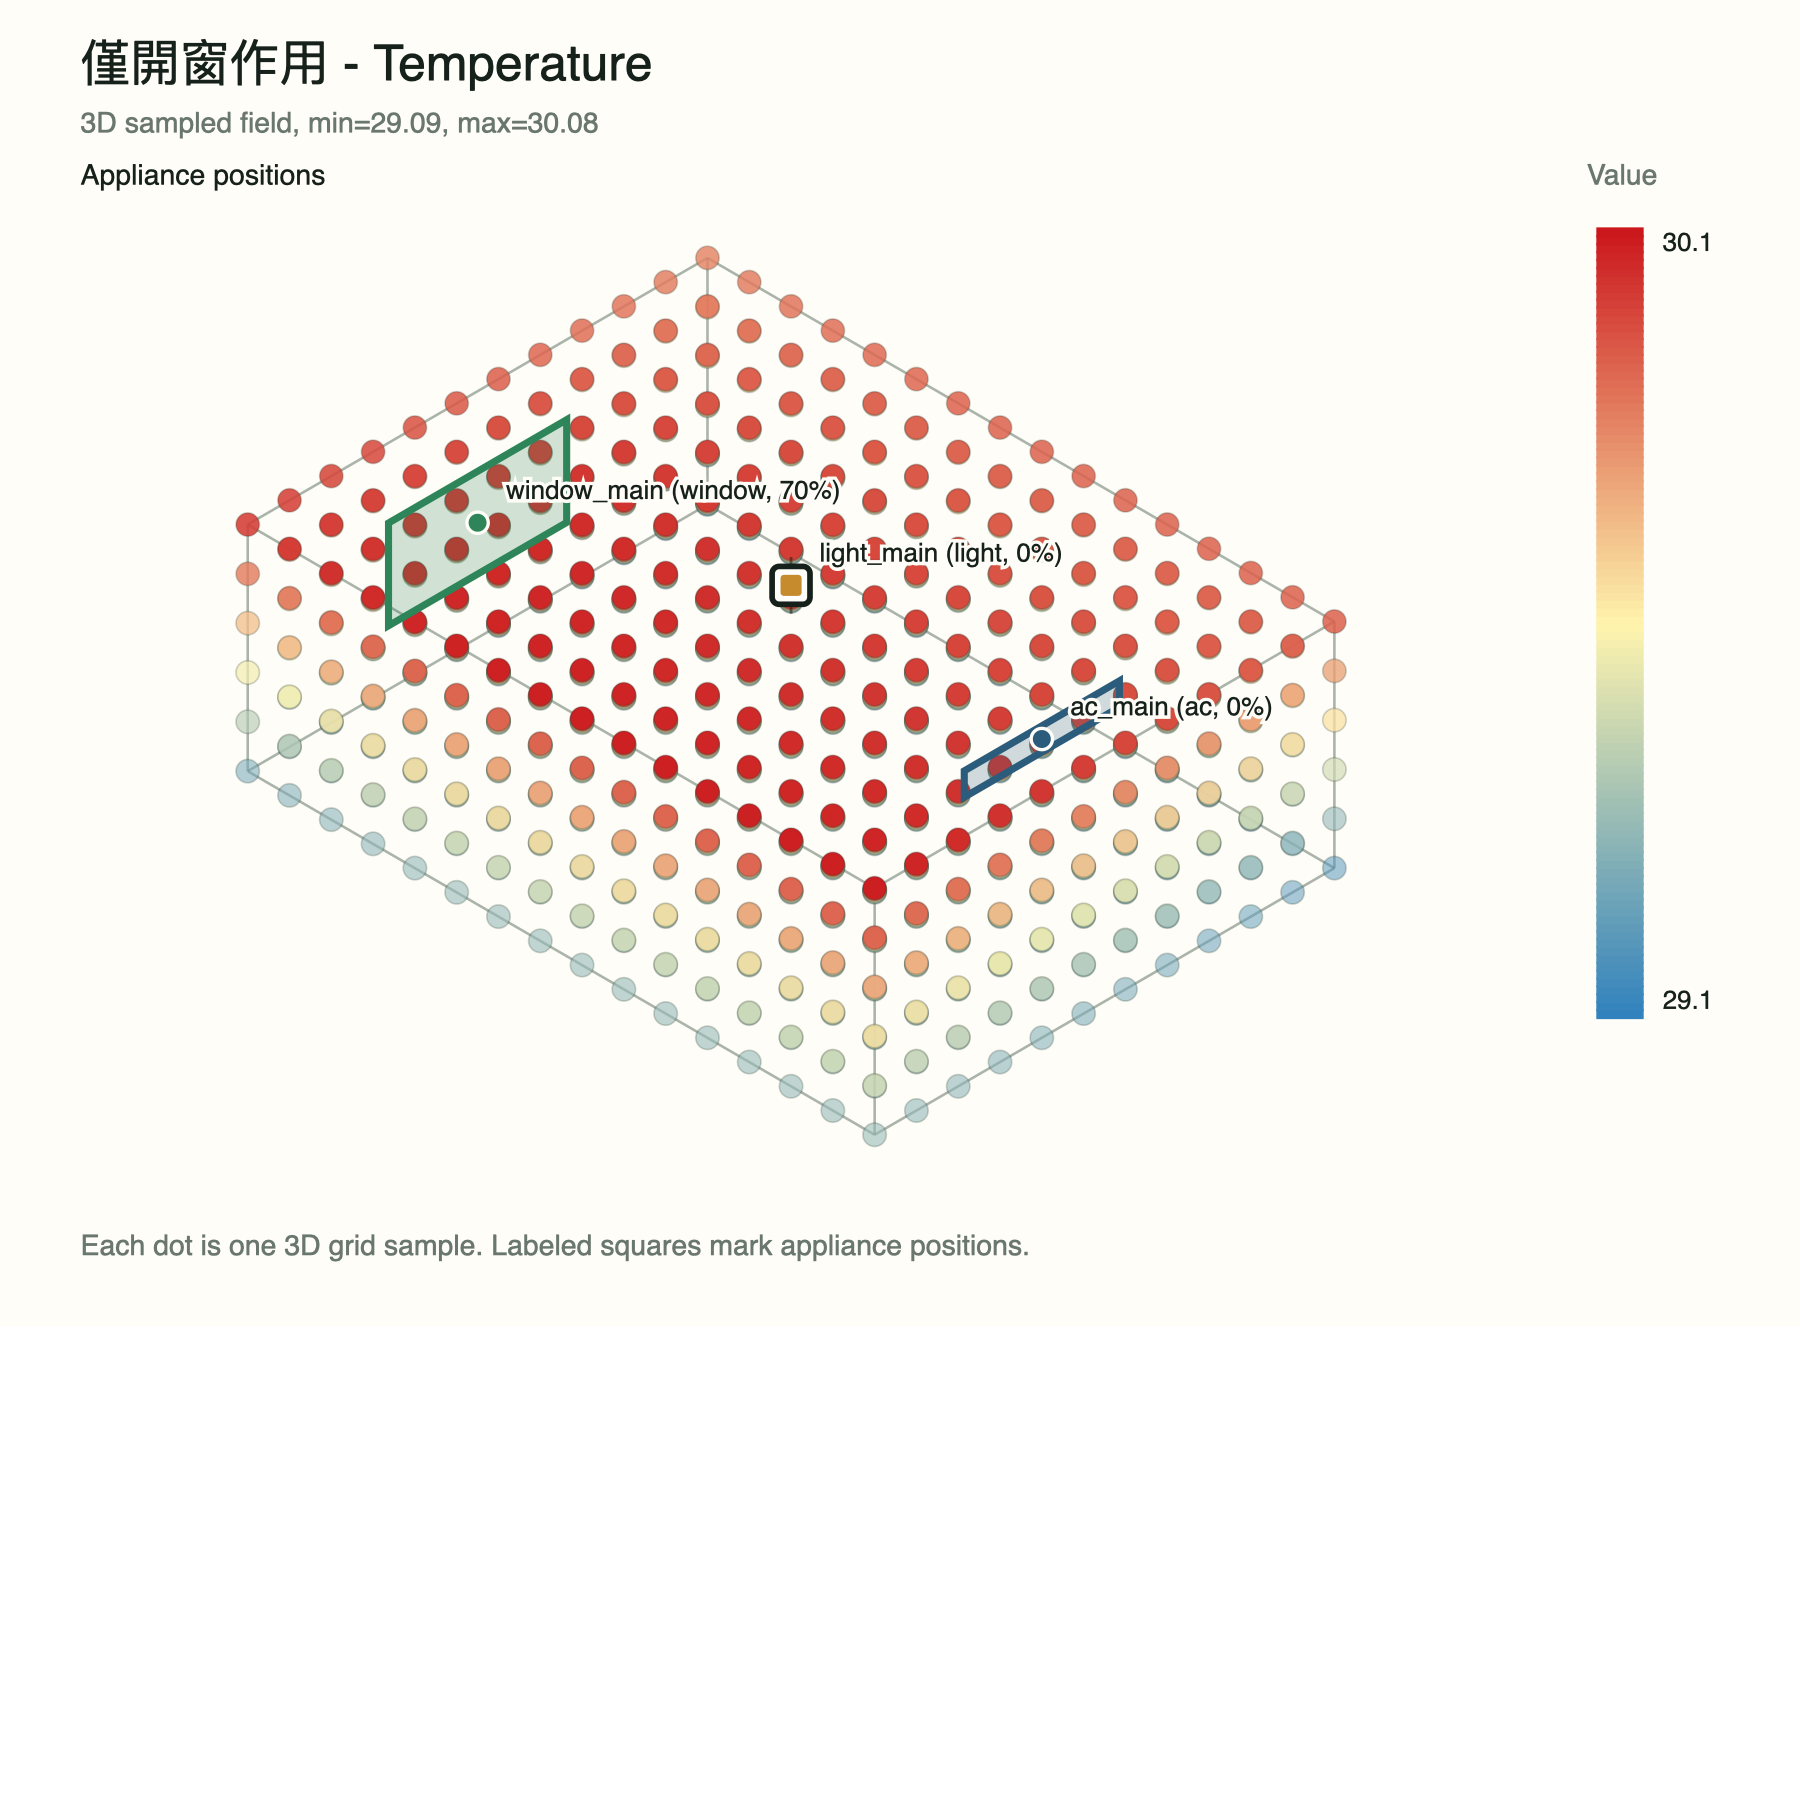
\includegraphics[width=0.83\textwidth]{assets/fig_5_6_window_only_temp_3d.png}
\par\smallskip
{\small 圖 5-6 僅開窗（window\textbackslash{}\_\allowbreak{}only）溫度場 3D 點雲。靠窗區域溫度最高，造成區域溫度梯度。可與 all\textbackslash{}\_\allowbreak{}active 情境對比，觀察冷氣介入後對窗邊高溫的抑制效果。}
\end{figure}

\begin{figure}[htbp]
\centering
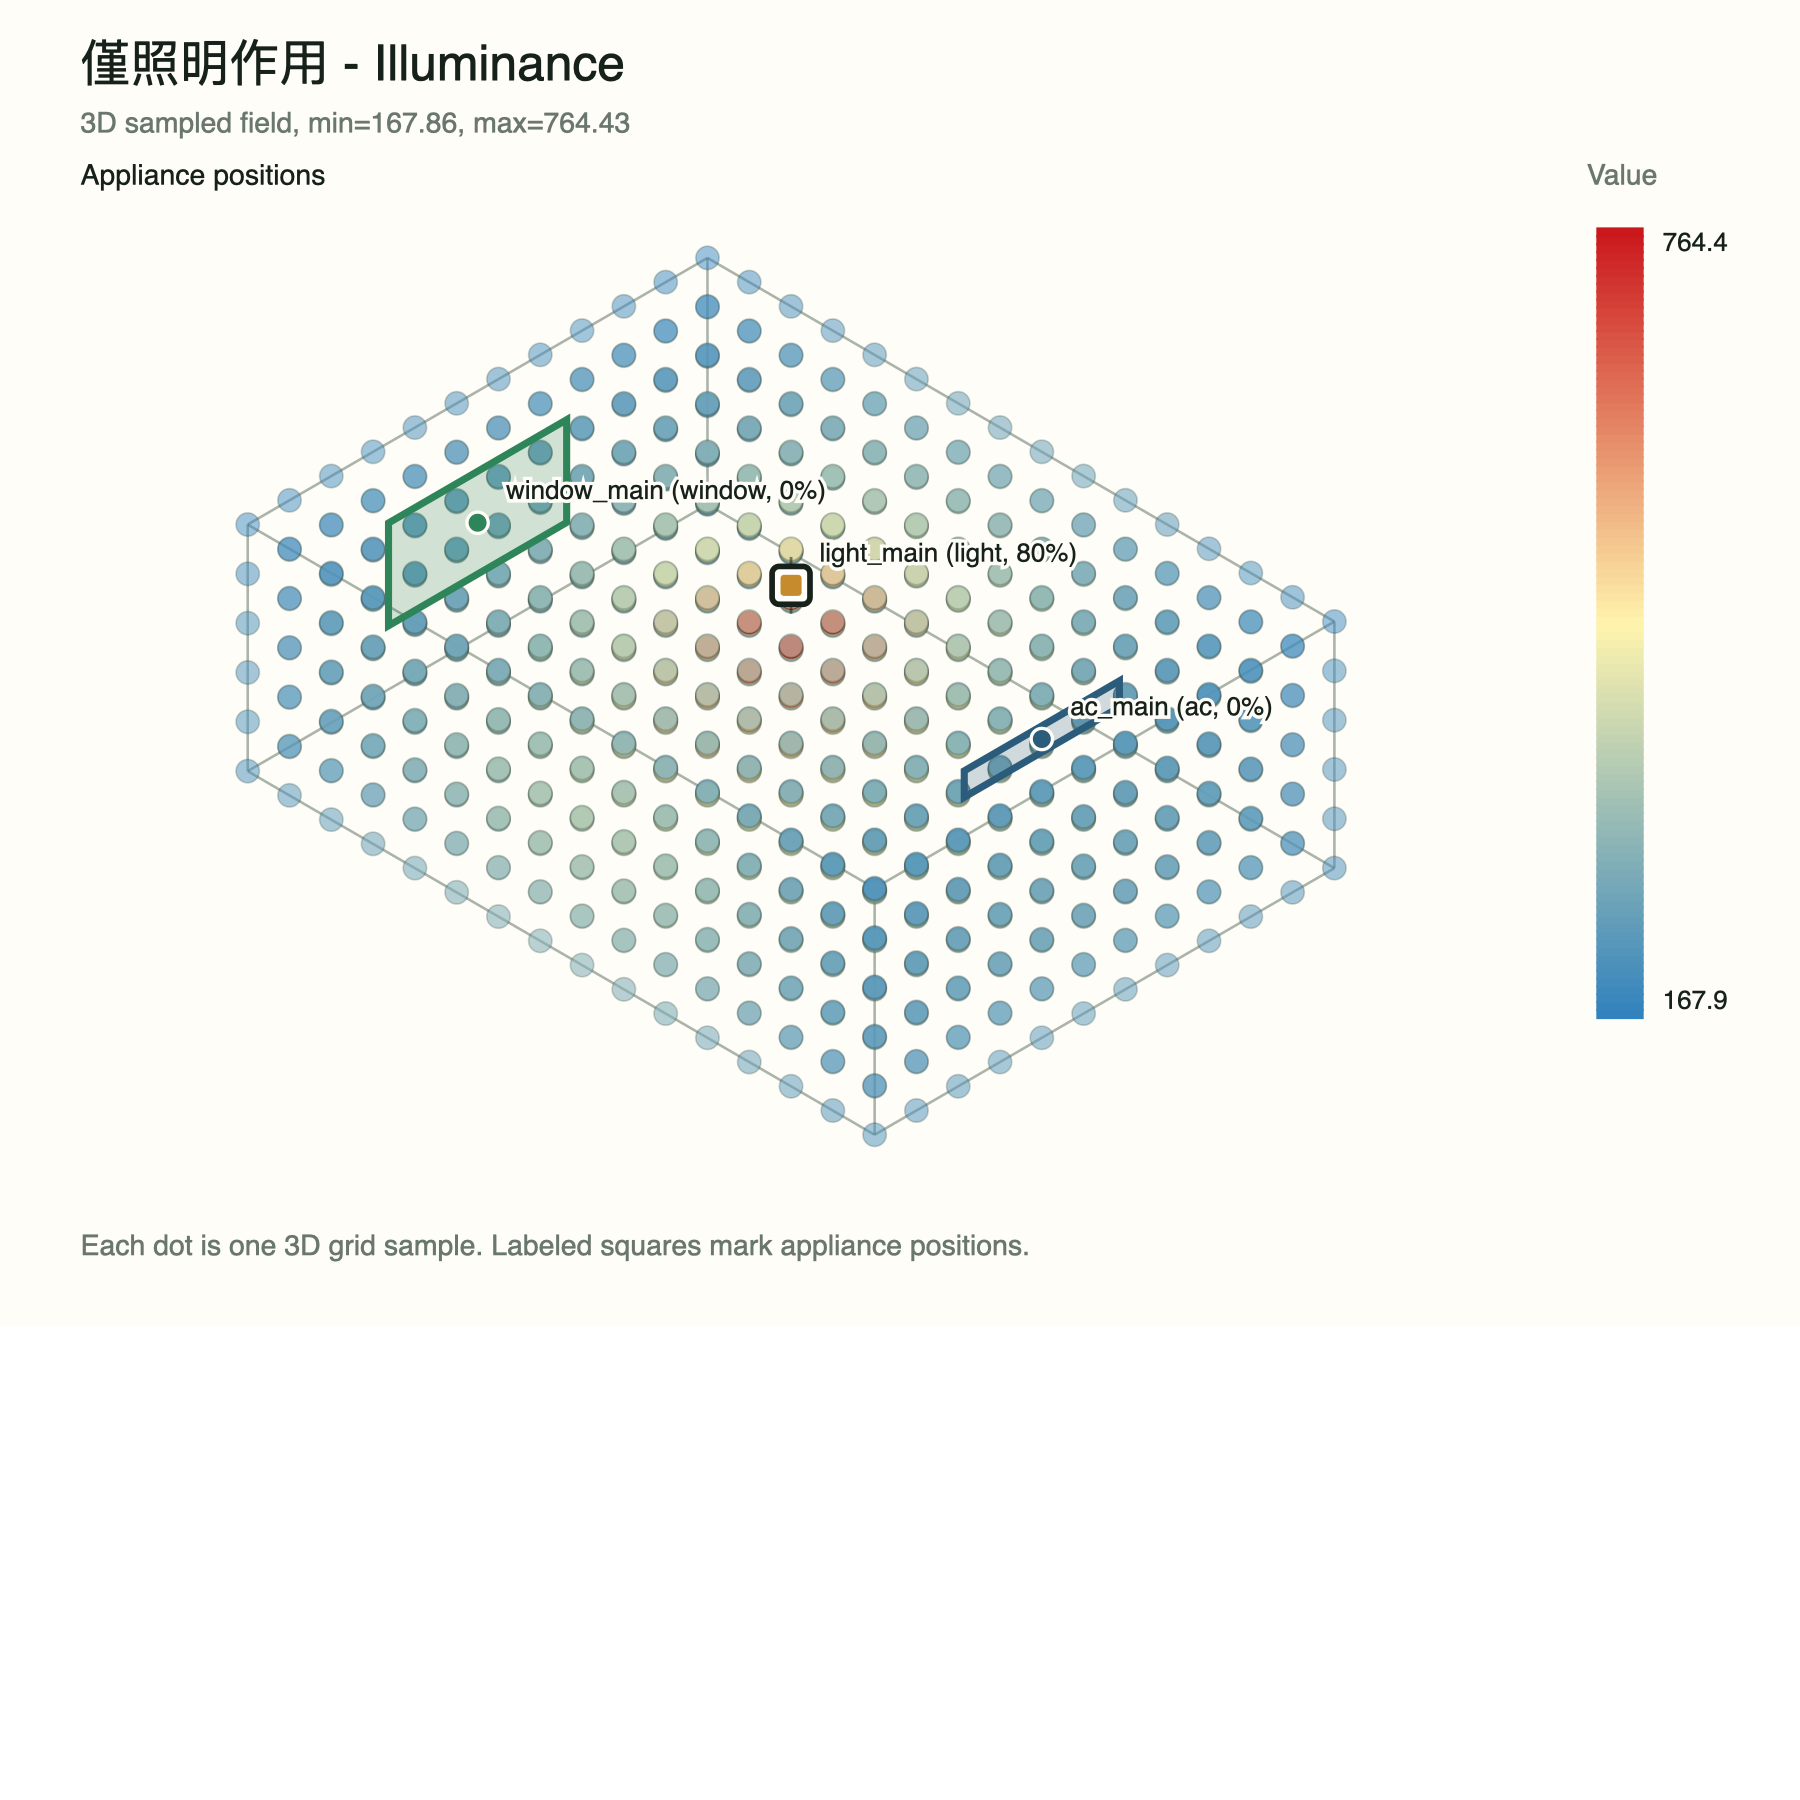
\includegraphics[width=0.83\textwidth]{assets/fig_5_7_light_only_illum_3d.png}
\par\smallskip
{\small 圖 5-7 僅燈具作用（light\textbackslash{}\_\allowbreak{}only）照度場 3D 點雲。燈具正下方照度最高，遠端補有少量的 single-bounce diffuse 回填；此情境也是 5.6 節 held-out 測試集之一。}
\end{figure}

\clearpage

\section*{第六章 結論與未來工作}
\addcontentsline{toc}{section}{第六章 結論與未來工作}

\subsection*{6.1 結論}

本研究建立一個面向非連網家電環境影響學習的單房間三因子空間數位孿生原型，針對 temperature、humidity 與 illuminance 的空間變化進行建模、校正與學習。透過 8 顆角落感測器、設備影響函數、active device power scale 校準、single-bounce diffuse reflection 與 trilinear 校正場，系統能估計房間內任意位置與指定區域的三因子狀態。模擬結果顯示，加入設備影響模型與照度反射近似後，在冷氣、窗戶與照明等情境下能提供較 IDW baseline 更可解釋且更精細的場估計；進一步加入只作用於 temperature / humidity residual trace 的 Fourier low-pass denoising 與 hybrid residual neural correction 後，held-out 情境的場重建誤差可再顯著下降。


此外，本研究將模型封裝為 MCP server，並提供 Gemma/Ollama bridge 與 web demo，使數位孿生不只是離線模擬程式，而是可被 AI client 或使用者互動查詢的工具化系統。整體成果符合研究目標：在有限感測器與非連網裝置條件下，學習裝置對空間環境的影響，並用於更準確的控制動作推薦。


在公開資料集 task-aligned benchmark 方面，本研究以 MAE、RMSE 與 Pearson Correlation 三項指標，對比 persistence 與 linear regression 兩個 baseline。結果顯示，本研究在複合任務（S3、C3）與長視窗（60min）溫度任務上具備明顯優勢：S3 複合任務中 persistence 的 Correlation 全為 0.000（因裝置切換導致趨勢中斷），而本研究仍維持 0.61–0.95 的有效趨勢預測能力；60min 視窗下溫度 MAE 與 RMSE 均為三者最低，說明物理結構在長視窗預測中優於純時序延續策略。劣勢則主要集中於短視窗純照度任務（15min）與外部資料濕度尺度不匹配：前者因照度在短時間內變化緩慢，persistence 策略本身即為有效 baseline；後者反映 SML2010 濕度量測尺度與本研究估計基準存在系統性偏差。此分析說明本研究的優勢來自模型結構對裝置影響的顯式建模，而非針對純時序預測最佳化。


另一項結論是，公開資料集並非不能使用，而是必須依資料本身支援的任務層級進行比較。對完整 3D 場重建，本研究目前仍以 canonical synthetic benchmark 作為主要依據；對 zone-level 響應、兩點時序響應與舒適度評分，則可分別利用相容的公開資料建立 task-aligned benchmark。此作法比直接宣稱所有資料集都能完整驗證本研究系統更嚴謹。


\subsection*{6.2 研究限制}

\begin{itemize}
\item 目前結果主要來自文獻參數與合理物理假設模擬，尚未加入大量真實房間資料。
\item 模型不處理多房間氣流、牆體熱容或完整流體動力學。
\item 濕度模型採簡化耦合，驗證強度低於溫度與照度；在外部資料集（SML2010）中存在系統性基準偏差，需進一步對齊量測尺度。
\item 短視窗（15min）純照度預測上，persistence baseline 因照度短期穩定性而具優勢，本研究的物理估計引入額外誤差。
\item 公開資料集多缺乏完整單房間幾何與 dense ground truth，因此無法直接作為 full-field benchmark。
\item MCP server 目前為本地 stdio 版本，尚未包含遠端部署、OAuth 或多使用者管理。
\item 控制功能為推薦排序，尚未進入自動閉環控制。
\end{itemize}

\subsection*{6.3 未來工作}

\begin{itemize}
\item 加入實體 ESP32 感測器資料，以校正與驗證模型參數。
\item 擴充自訂房間 JSON 輸入，使系統可支援不同房間尺寸與設備位置。
\item 為角落感測器加入照度量測通道（如光照感測元件），使角落光照資料可直接引入 trilinear residual correction，從而消除目前物理照度模型的系統性偏差，實現照度場的自我校正。
\item 加入更多環境變數，例如 CO2、PM2.5 或人體熱源。
\item 將 MCP server 擴充為遠端 HTTP MCP，並加入權限控管。
\item 進一步研究閉環控制，將推薦排序延伸為實際控制策略。
\item 加入長時間資料以學習季節性與日夜週期變化。
\item 以真實量測資料重新訓練與驗證 hybrid residual neural network，檢驗其在真實房間中的泛化能力。
\end{itemize}

\clearpage

\section*{參考文獻}
\addcontentsline{toc}{section}{參考文獻}

\begin{itemize}
\item [1] Per Bacher, Henrik Madsen, Identifying suitable models for the heat dynamics of buildings, Energy and Buildings, vol. 43, no. 7, pp. 1511-1522, 2011. DOI: 10.1016/j.enbuild.2011.02.005
\item [2] Petri Hietaharju, Mika Ruusunen, Kauko Leiviska, A Dynamic Model for Indoor Temperature Prediction in Buildings, Energies, vol. 11, no. 6, 1477, 2018. DOI: 10.3390/en11061477
\item [3] Gargya Gokhale, Bert Claessens, Chris Develder, Physics informed neural networks for control oriented thermal modeling of buildings, Applied Energy, vol. 314, 118852, 2022. DOI: 10.1016/j.apenergy.2022.118852
\item [4] E. J. Teshome, F. Haghighat, Zonal Models for Indoor Air Flow - A Critical Review, International Journal of Ventilation, vol. 3, no. 2, pp. 119-129, 2004. DOI: 10.1080/14733315.2004.11683908
\item [5] Boris Huljak, Juan A. Acero, Zin H. Kyaw, Francisco Chinesta, Hybrid models for simulating indoor temperature distribution in air-conditioned spaces, Frontiers in Built Environment, vol. 11, 1690062, 2025. DOI: 10.3389/fbuil.2025.1690062
\item [6] Ahmed Megri, Yao Yu, Rui Miao, Xiaoou Hu, A new dynamic zOnal model with air-diffuser (DOMA) - Application to thermal comfort prediction, Indoor and Built Environment, vol. 31, no. 7, pp. 1738-1757, 2022. DOI: 10.1177/1420326X211060486
\item [7] Andres Sebastian Cespedes-Cubides, Muhyiddine Jradi, A review of building digital twins to improve energy efficiency in the building operational stage, Energy Informatics, vol. 7, article 11, 2024. DOI: 10.1186/s42162-024-00313-7
\item [8] Weixin Qian, Chenxi Li, Hu Gao, Lei Zhuang, Yanyu Lu, Site Hu, Jing Liu, Estimating indoor air temperature and humidity distributions by data assimilation with finite observations: Validation using an actual residential room, Building and Environment, vol. 269, 112495, 2025. DOI: 10.1016/j.buildenv.2024.112495
\item [9] Y. Lisa Chen, Jin Wen, Application of zonal model on indoor air sensor network design, Proceedings of SPIE, vol. 6529, 652911, 2007. DOI: 10.1117/12.716356
\item [10] D. Shepard, A Two-Dimensional Interpolation Function for Irregularly-Spaced Data, Proceedings of the 1968 ACM National Conference, pp. 517-524, 1968.
\item [11] Model Context Protocol, Model Context Protocol Documentation, https://modelcontextprotocol.io/ , accessed 2026-04-10.
\item [12] Gopal Chitalia, Manisa Pipattanasomporn, CU-BEMS, smart building electricity consumption and indoor environmental sensor datasets, Scientific Data, vol. 7, article 290, 2020. DOI: 10.1038/s41597-020-00582-3
\item [13] Luis Candanedo, Appliances Energy Prediction [Dataset], UCI Machine Learning Repository, 2017. DOI: 10.24432/C5VC8G
\item [14] Pablo Romeu-Guallart, Francisco Zamora-Martinez, SML2010 [Dataset], UCI Machine Learning Repository, 2014. DOI: 10.24432/C5RS3S
\item [15] Luis Candanedo, Occupancy Detection [Dataset], UCI Machine Learning Repository, 2016. DOI: 10.24432/C5X01N
\item [16] Kamilla Heimar Andersen, Hicham Johra, Anna Marszal-Pomianowska, Per Kvols Heiselberg, Henrik N. Knudsen, Dataset of room-level indoor environmental quality measurements and occupancy ground truth for five residential apartments in Denmark [Dataset], Zenodo, 2024. DOI: 10.5281/zenodo.10761326
\item [17] V. Foldvary Licina, T. Cheung, H. Zhang, R. de Dear, T. Parkinson, E. Arens, et al., Development of the ASHRAE Global Thermal Comfort Database II, Building and Environment, vol. 142, pp. 502-512, 2018. DOI: 10.1016/j.buildenv.2018.06.022
\item [18] G. Chinazzo, J. Wienold, M. Andersen, Influence of indoor temperature and daylight illuminance on visual perception, Lighting Research and Technology, vol. 52, no. 8, pp. 998-1020, 2020. DOI: 10.1177/1477153519859609
\item [19] G. Chinazzo, J. Wienold, M. Andersen, Daylight affects human thermal perception, Scientific Reports, vol. 9, article 13695, 2019. DOI: 10.1038/s41598-019-48963-y
\item [20] Lan et al., Experimental study on the impact of indoor lighting and thermal environment on university students' learning performance in summer, Energy and Buildings, vol. 331, 115774, 2025. DOI: 10.1016/j.enbuild.2025.115774
\item [21] K. Kuwahara et al., Studying the Indoor Environment and Comfort of a University Laboratory: Air-Conditioning Operation and Natural Ventilation Used as a Countermeasure against COVID-19, Buildings, vol. 12, no. 7, 953, 2022. DOI: 10.3390/buildings12070953
\item [22] Yan Zhou, Jianmin Cai, Yiwen Xu, Indoor environmental quality and energy use evaluation of a three-star green office building in China with field study, Journal of Building Physics, vol. 45, no. 2, pp. 163-190, 2021. DOI: 10.1177/1744259120944604
\item [23] Z. Wang, Q. Xue, Y. Ji, Z. Yu, Indoor environment quality in a low-energy residential building in winter in Harbin, Building and Environment, vol. 135, pp. 194-201, 2018. DOI: 10.1016/j.buildenv.2018.03.012
\item [24] Y. Geng, B. Lin, Y. Zhu, Comparative study on indoor environment quality of green office buildings with different levels of energy use intensity, Building and Environment, vol. 168, 106482, 2020. DOI: 10.1016/j.buildenv.2019.106482
\item [25] J. Lee et al., A Comparative Field Study of Indoor Environment Quality and Work Productivity between Job Types in a Research Institute in Korea, International Journal of Environmental Research and Public Health, vol. 19, no. 21, 14332, 2022. DOI: 10.3390/ijerph192114332
\end{itemize}

\clearpage

\section*{附錄 A：原型執行方式}
\addcontentsline{toc}{section}{附錄 A：原型執行方式}

\begin{lstlisting}[basicstyle=\footnotesize\ttfamily,breaklines=true,columns=flexible]
python3 scripts/run_demo.py
python3 scripts/run_window_matrix.py
python3 scripts/run_hybrid_residual_experiment.py
python3 scripts/run_web_demo.py
python3 scripts/run_mcp_server.py
\end{lstlisting}

\section*{附錄 B：Web Demo 操作}
\addcontentsline{toc}{section}{附錄 B：Web Demo 操作}

\begin{itemize}
\item 左側 checkbox 控制 ac\_\allowbreak{}main、window\_\allowbreak{}main 與 light\_\allowbreak{}main。
\item 3D 預覽可拖曳旋轉，滾輪縮放。
\item Metric checkbox 可切換 temperature、humidity 與 illuminance。
\item 左側 Indoor Baseline 可直接調整室內基準溫度、濕度與照度。
\item 左側 Estimator toggle 可切換主模型與 hybrid residual corrected field。
\item 窗戶區可選季節、天氣與時段 preset，並手動覆寫外部溫度與開窗比例。
\item 時間軸可播放從啟動到接近準穩態的變化。
\item Point Sample 可查詢任意座標的三因子估計值。
\end{itemize}

\end{document}
